%%=======================================
%  WHUT Bachelor Thesis v 0.1b
%  
%  Tsao Yu
%  tsaoyu@tsaoyu.com
%  Last Modify Date Feb.6,2014
%%=======================================
\documentclass[cs4size,a4paper]{ctexart}
%\usepackage[scheme = plain]{ctex} %只提供中文支持,不改变版式风格

 %目录显示chapter层次
\makeatletter
\def\@bfdottedtocline#1#2#3#4#5{%
	\ifnum #1>\c@tocdepth \else
	\vskip \z@ \@plus.2\p@
	{\leftskip #2\relax \rightskip \@tocrmarg \parfillskip -\rightskip
		\parindent #2\relax\@afterindenttrue
		\interlinepenalty\@M
		\leavevmode \bfseries
		\@tempdima #3\relax
		\advance\leftskip \@tempdima \null\nobreak\hskip -\leftskip
		{#4}\normalfont\nobreak
		\leaders\hbox{$\m@th
			\mkern \@dotsep mu\hbox{.}\mkern \@dotsep
			mu$}\hfill
		\nobreak
		\hb@xt@\@pnumwidth{\hfil\normalfont \normalcolor #5}%
		\par}%
	\fi}
\renewcommand*\l@section{\@bfdottedtocline{0}{0em}{1.5em}}
\makeatother

%\documentclass[cs4size,a4paper]{ctexrep} %有chapter层次 
\setcounter{tocdepth}{2}%目录显示2层  
%==================== 数学符号公式 ============
\usepackage{polynom}
\usepackage[super,square,comma,sort&compress,numbers]{natbib}%参考文献上标,方框
\usepackage{amsmath}                 % AMS LaTeX宏包
%\usepackage{amssymb}                % 用来排版漂亮的数学公式
%\usepackage{amsbsy}
\usepackage{booktabs}                %三线表
\usepackage[style=1]{mdframed}
\usepackage{enumitem}                %列表环境
\usepackage{amsthm}
\usepackage{amsfonts}
\usepackage{mathrsfs}                % 英文花体字 体
\usepackage{bm}                      % 数学公式中的黑斜体
\usepackage{bbding,manfnt}           % 一些图标,如 \dbend
\usepackage{lettrine}                % 首字下沉,命令\lettrine
\def\attention{\lettrine[lines=2,lraise=0,nindent=0em]{\large\textdbend\hspace{1mm}}{}}
\usepackage{longtable}
\usepackage[toc,page]{appendix}
\usepackage{geometry}                % 页边距调整
\geometry{top=2.5cm,bottom=2.0cm,left=2.5cm,right=2.0cm}
%\usepackage{relsize}                % 调整公式字体大小:\mathsmaller,\mathlarger
%\usepackage{caption2}               % 浮动图形和表格标题样式
%====================系统本地华文中宋字体==================
%\setCJKfamilyfont{hwzs}{STZhongsong}   %字体部分使用
%\newcommand{\stzs}{\CJKfamily{hwzs}}
%\setmainfont{Times New Roman}        %全局英文使用time new roman
%====================公式按章编号==========================
\numberwithin{equation}{section}
\numberwithin{table}{section}
\numberwithin{figure}{section}
%================= 基本格式预置 ===========================
\usepackage{fancyhdr}
\pagestyle{fancy}                    %采用fancy页眉页脚风格
%\fancyhf{}                           %清除所有页眉页脚
%\fancyhead[C]{\zihao{5}  \songti  同济大学中德学院课程报告 }	%设置页眉
\fancyfoot[C]{~\zihao{5} \thepage~}						%设置页脚
\renewcommand{\headrulewidth}{0.65pt} 
%\CTEXsetup[format={\centering\bfseries\zihao{-2}},name={第, 章}]{section}
%取消你用section设置章格式的用法,恢复节格式。
\CTEXsetup[format={\raggedright\bfseries\zihao{3}}]{section}
%format 用来控制章节标题德全局格式,nameformat则是控制章节名词和编号格式,不包括后面的标题内容(比如第1章 目录,只控制第1章)
%\CTEXsetup[nameformat={\bfseries\zihao{3}}]{section}
\CTEXsetup[nameformat={\bfseries\zihao{3}}]{subsection}
\CTEXsetup[nameformat={\bfseries\zihao{4}}]{subsubsection}
%
%================== 图形支持宏包 =========================
\usepackage{subfigure}
\usepackage{array}
\usepackage{tabularx}               %宽度调整的表格
\newcolumntype{Y}{>{\centering\arraybackslash}X}
\usepackage{varwidth}               %自动调整宽度
\usepackage{float}
\usepackage{graphicx}                % 嵌入png图像
\usepackage{color,xcolor}            % 支持彩色文本、底色、文本框等
\usepackage{hyperref}                % 交叉引用,生成超链接目录等
\hypersetup{hidelinks}               %隐藏链接,将目录、超链接红色等改为黑色。
\hypersetup{bookmarksnumbered=true}  %psfbookmark中显示章节编号
\usepackage{caption}                 %图表标题格式控制宏包
\captionsetup{labelsep=space}        %图的标签(图x-xx)和标题之间用空格
\captionsetup{figurewithin=section}
%==================== 源码和流程图 =====================
\usepackage{listings}                % 粘贴源代码
\usepackage{color}

\definecolor{dkgreen}{rgb}{0,0.6,0}
\definecolor{gray}{rgb}{0.5,0.5,0.5}
\definecolor{mauve}{rgb}{0.58,0,0.82}
%代码格式
\lstset{ %
	language=Octave,                % the language of the code
	basicstyle=\footnotesize,           % the size of the fonts that are used for the code
	numbers=left,                   % where to put the line-numbers
	numberstyle=\tiny\color{gray},  % the style that is used for the line-numbers
	stepnumber=2,                   % the step between two line-numbers. If it's 1, each line 
	% will be numbered
	numbersep=5pt,                  % how far the line-numbers are from the code
	backgroundcolor=\color{white},      % choose the background color. You must add \usepackage{color}
	showspaces=false,               % show spaces adding particular underscores
	showstringspaces=false,         % underline spaces within strings
	showtabs=false,                 % show tabs within strings adding particular underscores
	%frame=single,                   % adds a frame around the code
	rulecolor=\color{black},        % if not set, the frame-color may be changed on line-breaks within not-black text (e.g. commens (green here))
	tabsize=2,                      % sets default tabsize to 2 spaces
	captionpos=b,                   % sets the caption-position to bottom
	breaklines=true,                % sets automatic line breaking
	breakatwhitespace=false,        % sets if automatic breaks should only happen at whitespace
	title=\lstname,                   % show the filename of files included with \lstinputlisting;
	% also try caption instead of title
	keywordstyle=\color{blue},          % keyword style
	commentstyle=\color{dkgreen},       % comment style
	stringstyle=\color{mauve},         % string literal style
	escapeinside={\%*}{*)},            % if you want to add LaTeX within your code
	morekeywords={*,...}               % if you want to add more keywords to the set
}
\usepackage{tikz}                    
\usepackage{tikz-3dplot}
\usetikzlibrary{shapes,arrows,positioning}
%=================== 自定义插图命令=======================
%插入水平图2个,分别标图注
\newcommand{\insTwoGraphonSg}[6]{	
	\begin{figure}[H]
		\centering
		\begin{minipage}[t]{0.45\linewidth}
			\centering
			\includegraphics[width=\linewidth]{#1}
			\caption{#2}
			\label{fig:#3}
		\end{minipage}
		\quad
		\begin{minipage}[t]{0.45\linewidth}
			\centering
			\includegraphics[width=\linewidth]{#4}
			\caption{#5}
			\label{fig:#6}
		\end{minipage}
	\end{figure}}

%插入矩阵图2X2,一个图注加4哥分图注
%\newcommand{\insFourGrapSg}[14]{\begin{figure}[H]
%		\centering
%		\subfigure[#1]{%
%			\includegraphics[width=0.4\linewidth]{#2}
%			\label{fig:#3}}
%		\quad
%		\subfigure[#4]{%
%			\includegraphics[width=0.4\linewidth]{#5}
%			\label{fig:#6}}
%		\subfigure[#7]{%
%			\includegraphics[width=0.4\linewidth]{#8}
%			\label{fig:#9}}
%		\quad
%		\subfigure[传统的接收节点]{%
%			\includegraphics[width=0.4\linewidth]{figure/can_node1}
%			\label{fig:node_subfigure4}}
%		%
%		\caption{数据加密系统的CAN节点与传统的CAN节点对比}
%		\label{fig:node_figure}
%%%	\end{figure}}

%==================列表命令自定义================%
%定义新的列表环境
%带括号标记,第一行缩进
\newlist{mylist}{enumerate}{1}
\setlist[mylist,1]{fullwidth,itemindent=\parindent,labelsep=0pt,partopsep=0pt,parsep=0pt,topsep=0pt,itemsep=0pt,label=\arabic*)}
%带括号标记,全部缩进
\newlist{mylist1}{enumerate}{1}
\setlist[mylist1,1]{fullwidth,leftmargin=3em,labelwidth=1em,labelsep=0pt,itemindent=0pt,partopsep=0pt,parsep=0pt,topsep=0pt,itemsep=0pt,label=\arabic*)}
%黑点标记,全部缩进
\newenvironment{mylist2}{\begin{itemize}[leftmargin=3em,partopsep=0pt,parsep=0pt,topsep=0pt,itemsep=0pt]}{\end{itemize}}

%===================表格命令自定义===============%
%以下是三线表格命令
%\begin{table}[H]
%	\setlength{\abovecaptionskip}{-10pt}   
%	\setlength{\belowcaptionskip}{0pt}   %这2行是为了使表标题与表格距离适当
%	\caption{AES密钥长度与算法执行轮数的关系}
%	\begin{center}
%		\begin{tabularx}{\textwidth}{YY}
%			\toprule  
%			密钥长度 & 算法执行轮数$n_{r}$  \\ 
%			\midrule 
%			128位 & 10  \\ 
%			192位 & 12 \\ 
%			256位 & 14 \\  
%			\bottomrule
%		\end{tabularx} 
%	\end{center}
%	\label{tb:key_round}
%\end{table}
%\begin{figure}[H]
%	\centering
%	\includegraphics[width=\linewidth]{figure/bit_stuff}
%	\caption{位填充示例}
%	\label{fig:bit_stuff}
%\end{figure}
%如图\ref{fig:bit_stuff}所示。
%===================   正文开始    ===================
\begin{document}
\bibliographystyle{gbt7714-2005}     %论文引用格式
%===================  定理类环境定义 ===================
\newtheorem{example}{例}              % 整体编号
\newtheorem{algorithm}{算法}
\newtheorem{theorem}{定理}[section]           % 按 section 编号
\newtheorem{definition}{\hskip 2em 定义}[section]
\newtheorem{axiom}{公理}[section]
\newtheorem{property}{性质}
\newtheorem{proposition}{命题}
\newtheorem{lemma}{引理}[section]
\newtheorem{corollary}{推论}
\newtheorem{remark}{注解}
\newtheorem{condition}{条件}
\newtheorem{conclusion}{结论}
\newtheorem{assumption}{假设}
%==================重定义 ===================
\renewcommand{\contentsname}{目录}     
\renewcommand{\abstractname}{摘要} 
\renewcommand{\refname}{参考文献}     
\renewcommand{\indexname}{索引}
\renewcommand{\figurename}{图}
\renewcommand{\tablename}{表}
\renewcommand{\appendixname}{附录}
\renewcommand{\proofname}{证明}
\renewcommand{\algorithm}{算法} 
%============== 封皮和前言 =================
%===============  封面  =================
\smallskip
\begin{center}
%\begin{figure}[!th]
%\centering
%\includegraphics[width=0.7\linewidth]{figure/SchoolName}
%\end{figure}

\begin{figure}[H]
	\centering
	\begin{minipage}[t]{0.4\linewidth}
		\centering
		
\includegraphics[width=\linewidth]{figure/header_logo_cdhk}
	\end{minipage}
    \quad
	\begin{minipage}[t]{0.4\linewidth}
		\centering
		
\includegraphics[width=\linewidth]{figure/header_logo_tongji}
	\end{minipage}
\end{figure}
\vspace*{2.0cm}
{\zihao{1}  同济大学中德学院课程报告} \\
\vspace*{2.1cm}
 {\zihao{2}  基于PHP的动态网站说明书 }\\
\vspace*{6.0cm}

\begin{tabular}{cc}
\zihao{3}  学\qquad 院:&\underline{\makebox[7cm][c]{\zihao{3}中德学院}} \\ 
\\
 \zihao{3}  课\qquad 程:&\underline{\makebox[7cm][c]{\zihao{3}软件技术基础}} \\ 
 \\
 \zihao{3}专业年级: & \underline{\makebox[7cm][c]{\zihao{3}车辆工程专业16级}} \\ 
 \\
 \zihao{3}学生姓名: & \underline{\makebox[7cm][c]{\zihao{3}毛威}} \\ 
 \\
 \zihao{3}指导教师: & \underline{\makebox[7cm][c]{\zihao{3}沈斌教授}} \\ 
 \\
\end{tabular} 
\end{center}
\thispagestyle{empty}
\clearpage
%=====================原创性声明===========
%\begin{center}
%\zihao{-2} \textbf{学位论文原创性声明}
%\end{center}
%
%本人郑重声明:所呈交的论文是本人在导师的指导下独立进行研究所取得的研究成果。除了文中特别加以标注引用的内容外,本论文不包括任何其他个人或集体已经发表或撰写的成果作品。本人完全意识到本声明的法律后果由本人承担。 
%\begin{flushright}
%\zihao{4} 作者签名:\qquad ~~~\\
%
%年\qquad 月\qquad 日
%\end{flushright}
%\vskip 2cm
%\begin{center}
%\zihao{-2} \textbf{学位论文版权使用授权书}
%\end{center}
%
%本学位论文作者完全了解学校有关保障、使用学位论文的规定,同意学校保留并向有关学位论文管理部门或机构送交论文的复印件和电子版,允许论文被查阅和借阅。本人授权省级优秀学士论文评选机构将本学位论文的全部或部分内容编入有关数据进行检索,可以采用影印、缩印或扫描等复制手段保存和汇编本学位论文。\smallskip
%
%本学位论文属于
%\begin{tabular}[t]{l}
%1、保密$ \Box$,在~~~年解密后适用本授权书  \\ 
%2、不保密$ \Box$  \\ 
%\end{tabular} \\
%\begin{center}
%(请在以上相应方框内打“$\surd”$)
%\end{center}
%\begin{flushright}
%\zihao{4} 作者签名:  \quad\quad\quad\quad 年 \quad  月  \quad  日\\
%导师签名:   \quad\quad\quad\quad 年 \quad  月 \quad   日\\
%\end{flushright}
%\thispagestyle{empty}  %清除页眉页脚
%\clearpage             %换页

                          %input不会自动换页
%\pagestyle{plain}                           %摘要开始页脚中间页码
%\pagenumbering{arabic}                       %摘要开始页脚中间页码大写罗马数字
%egdsg                     %include 自动换页
\pagestyle{empty}                           %清除页眉页脚及页码计数器
\tableofcontents                            %输出目录
\thispagestyle{empty}
\clearpage
%============== 论文正文   =================
\pagestyle{fancy}
\pagenumbering{arabic}  
%\setcounter{page}{0}
\section{网页设计原理}
\subsection{软件及语言}
设计动态网页所用软件如下:
\begin{mylist1}
  \item Internet Information Services (IIS)。Web服务器软件,可以执行PHP语言。
  \item Dreamweaver CS6。它是一种有可视化编辑界面,用于制作并编辑网站的网页设计软件。
  \item PhpStudy for IIS 2014。它是一个集成IIS+PhpMyAdmin
  +PHP+MySQL于一体PHP调试环境程序集成包,。
  \item MySQLWorkbench。可视化MySQL数据库建模软件\cite{Ullman-418}。
\end{mylist1}

设计网页使用的语言如下:
\begin{mylist1}
\item 服务器端(后台)语言:PHP。
\item 浏览器端(前端)语言:HTML 、JQuery。JQuery是JavaScript的一种封装,是一个快速、简洁的JavaScript框架。
\item 数据库查询计语言:SQL。
\end{mylist1}
\subsection{数据库建立}
本文设计的动态网页用来管理汽车产品及其零部件。每一个汽车产品对应自己的零部件,分别建立汽车产品和汽车零部件表单。汽车产品表单各个字段如表\ref{tb:prd}所示,其中$prd\_id$为汽车产品表的主键。
\begin{table}[H]
	\setlength{\abovecaptionskip}{-10pt}   
	\setlength{\belowcaptionskip}{0pt}   %这2行是为了使表标题与表格距离适当
	\caption{汽车产品表}
	\begin{center}
		\begin{tabularx}{\textwidth}{YY}
			\toprule  
			字段 & 示例  \\ 
			\midrule 
			$prd\_id$ & 2  \\ 
			$prd\_num$ & P16 \\ 
			$prd\_style$ & 	POLO 1.4L \\ 
			$prd\_name$ & 全新POLO2016款 自动风尚版 \\
			$prd\_manf$ & 上海大众汽车 \\
			$prd\_area$ & 上海嘉定 \\
			$prd\_price$ & 80000 \\
			\bottomrule
		\end{tabularx} 
	\end{center}
	\label{tb:prd}
\end{table}

零件表如表\ref{tb:prt}所示,其中的	$prt\_id$为零部件表的主键,而$car\_prod\_prd\_id $则为外键即汽车产品在零件表中的体现。
\begin{table}[H]
	\setlength{\abovecaptionskip}{-10pt}   
	\setlength{\belowcaptionskip}{0pt}   %这2行是为了使表标题与表格距离适当
	\caption{零部件表}
	\begin{center}
		\begin{tabularx}{\textwidth}{YY}
			\toprule  
			字段 & 示例  \\ 
			\midrule 
			$prt\_id$ & 26  \\ 
			$prt\_num$ & PL04 \\ 
			$car\_prod\_prd\_id $ & 2 \\ 
			$prt\_name$ & 上海大众POLO自动变速器 \\
			$prt\_manf$ & Aisin-AW公司车 \\
			$prt\_manfAdr$ & 日本 \\
			$prt\_price$ & 4000 \\
			\bottomrule
		\end{tabularx} 
	\end{center}
	\label{tb:prt}
\end{table}

本文网页的各个功能,只有已注册用户才能使用,所以本文还设计了用户信息表\ref{tb:user}。其中的密码($r\_pass$)字段值以密文存储。
\begin{table}[H]
	\setlength{\abovecaptionskip}{-10pt}   
	\setlength{\belowcaptionskip}{0pt}   %这2行是为了使表标题与表格距离适当
	\caption{用户信息表}
	\begin{center}
		\begin{tabularx}{\textwidth}{YY}
			\toprule  
			字段 & 示例  \\ 
			\midrule 
			$r\_id$ & 1 \\ 
			$r\_name$ & admin \\ 
			$r\_pass$ & 21232f297a57a5a743894a0e4a801fc3 \\ 
			$r\_date$ & 2016-12-17 \\
			\bottomrule
		\end{tabularx} 
	\end{center}
	\label{tb:user}
\end{table}

按照上述思路,在MySQLWorkbench中建立由汽车产品表(car\_prod)、零部件表(car\_part)和用户表(reg)组成的数据库。数据库模型如图\ref{fig:cardb}所示,一个汽车产品对应多个零件(即一对多关系数据库)。
\begin{figure}[H]
\centering
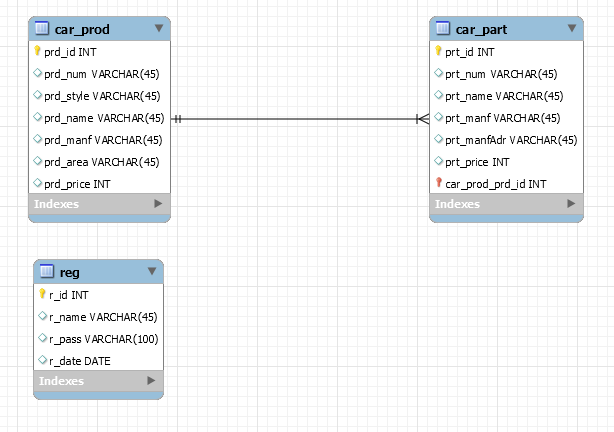
\includegraphics[width=0.9\linewidth]{figure/cardb}
\caption{汽车PDM数据库}
\label{fig:cardb}
\end{figure}
\subsection{动态网页结构}
本文设计的动态网页结构图\ref{fig:webStruk}所示。用户通过客户端浏览器(比如谷歌浏览器)向服务器(比如IIS)发出请求,可以实现对MySQL数据库中的数据进行操作(比如信息查询、删除、修改、添加和BOM表显示等)。
\begin{figure}[H]
\centering
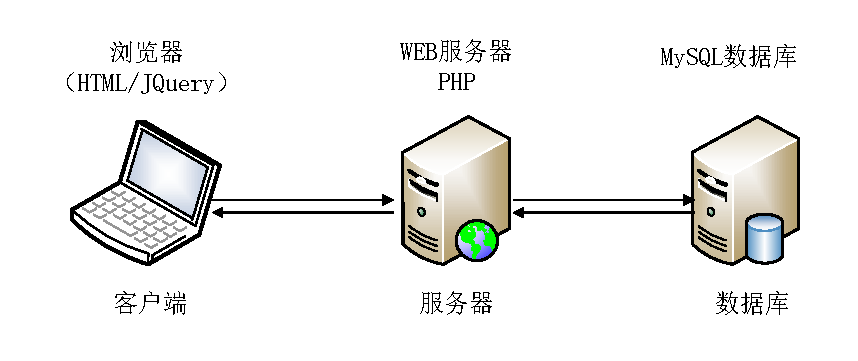
\includegraphics[width=1\linewidth]{figure/webStruk}
\caption{汽车PDM动态网页结构}
\label{fig:webStruk}
\end{figure}

\par~~~~~~~~~~

 网页在谷歌浏览器中的显示效果如图\ref{fig:index}所示。
\begin{figure}[H]
\centering
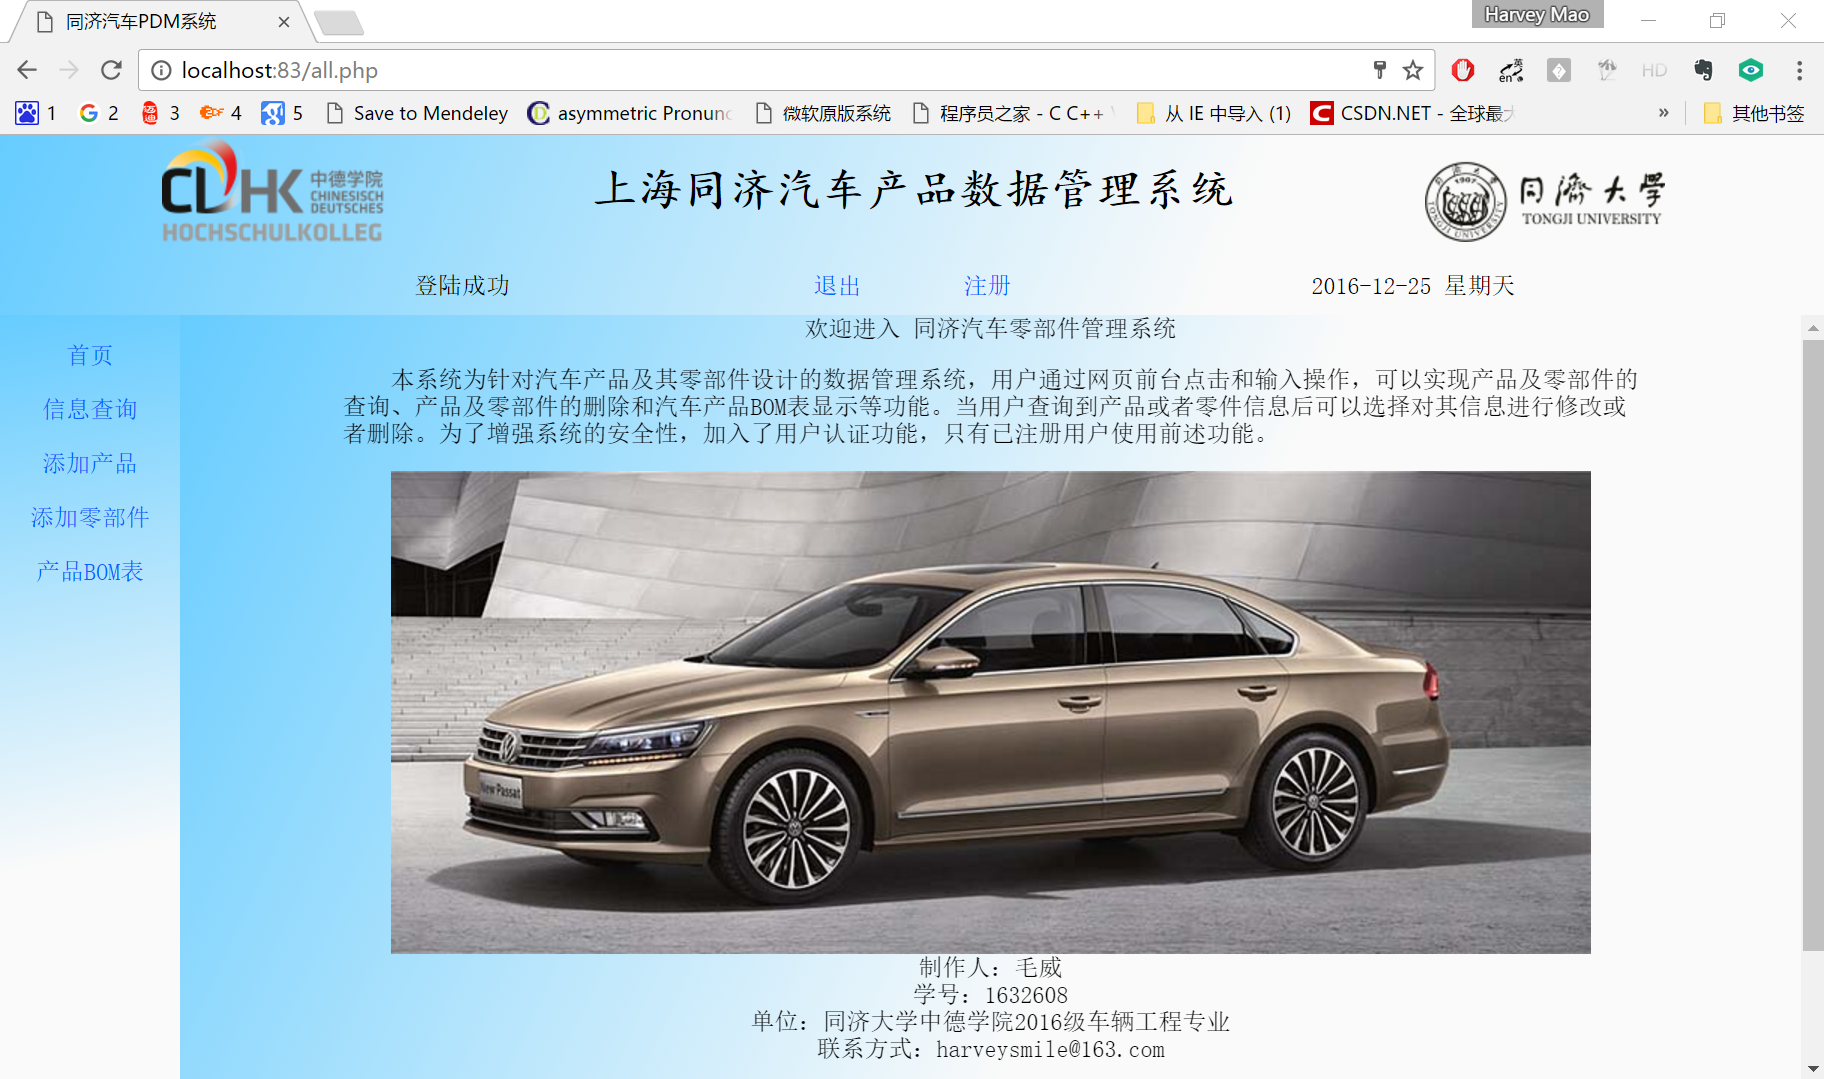
\includegraphics[width=0.9\linewidth]{figure/index}
\caption{汽车PDM动态网页}
\label{fig:index}
\end{figure}
 
站点文件结如图\ref{fig:webSite}下:
\begin{figure}[H]
\centering
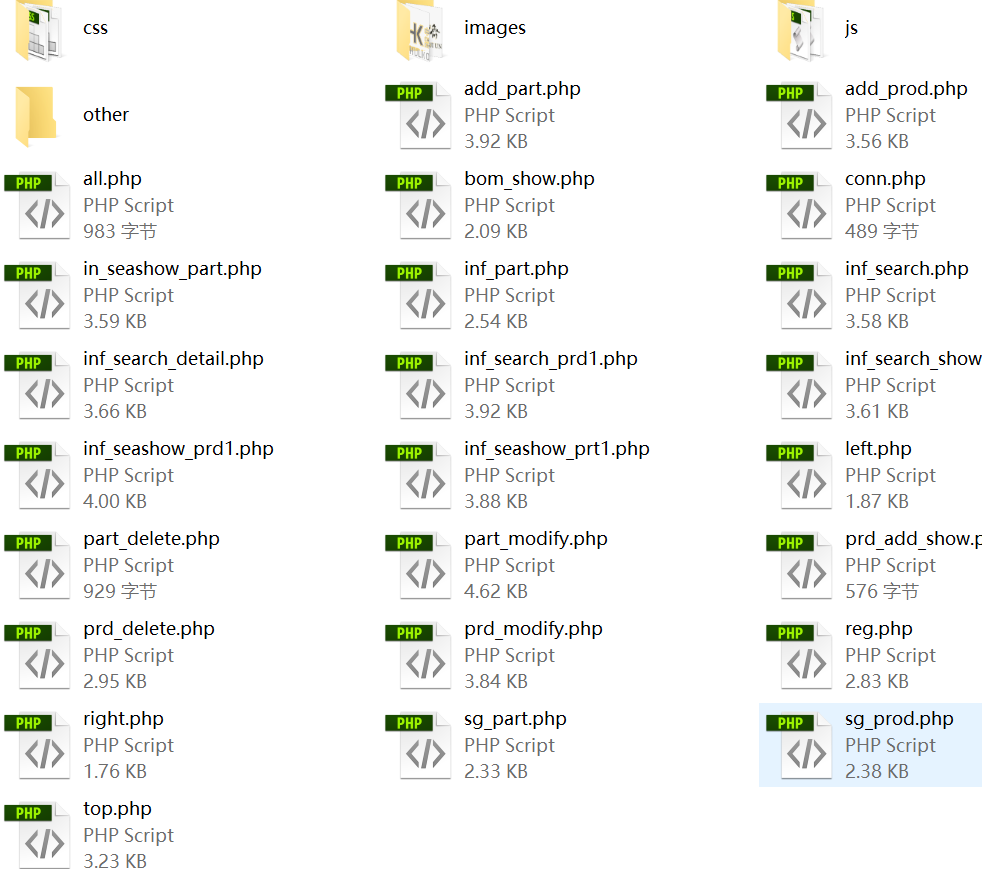
\includegraphics[width=0.8\linewidth]{figure/webSite}
\caption{汽车PDM站点}
\label{fig:webSite}
\end{figure}
%引入第一节
%\section{主要功能介绍}
该系统的主要功能有信息查询、产品添加、零件添加、BOM表显示和用户认证。具体功能架构如图\ref{fig:function}所示:
\begin{figure}[H]
\centering
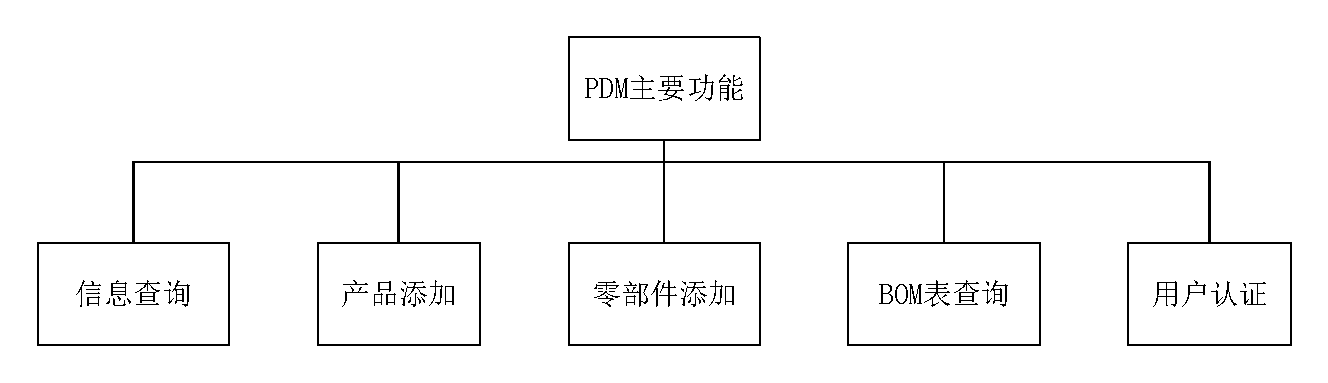
\includegraphics[width=0.9\linewidth]{figure/function.pdf}
\caption{PDM主要功能}
\label{fig:function}
\end{figure}

此外支持对数据汽车产品及零件的查询支持简单查询和高级查询;支持汽车附属零件信息的显示;支持对汽车产品及其零部件的修改和删除;支持通过BOM表显示整个PDM数据库的数据结构。

PDM系统的主界面如图\ref{fig:index1}所示。
\begin{figure}[H]
\centering
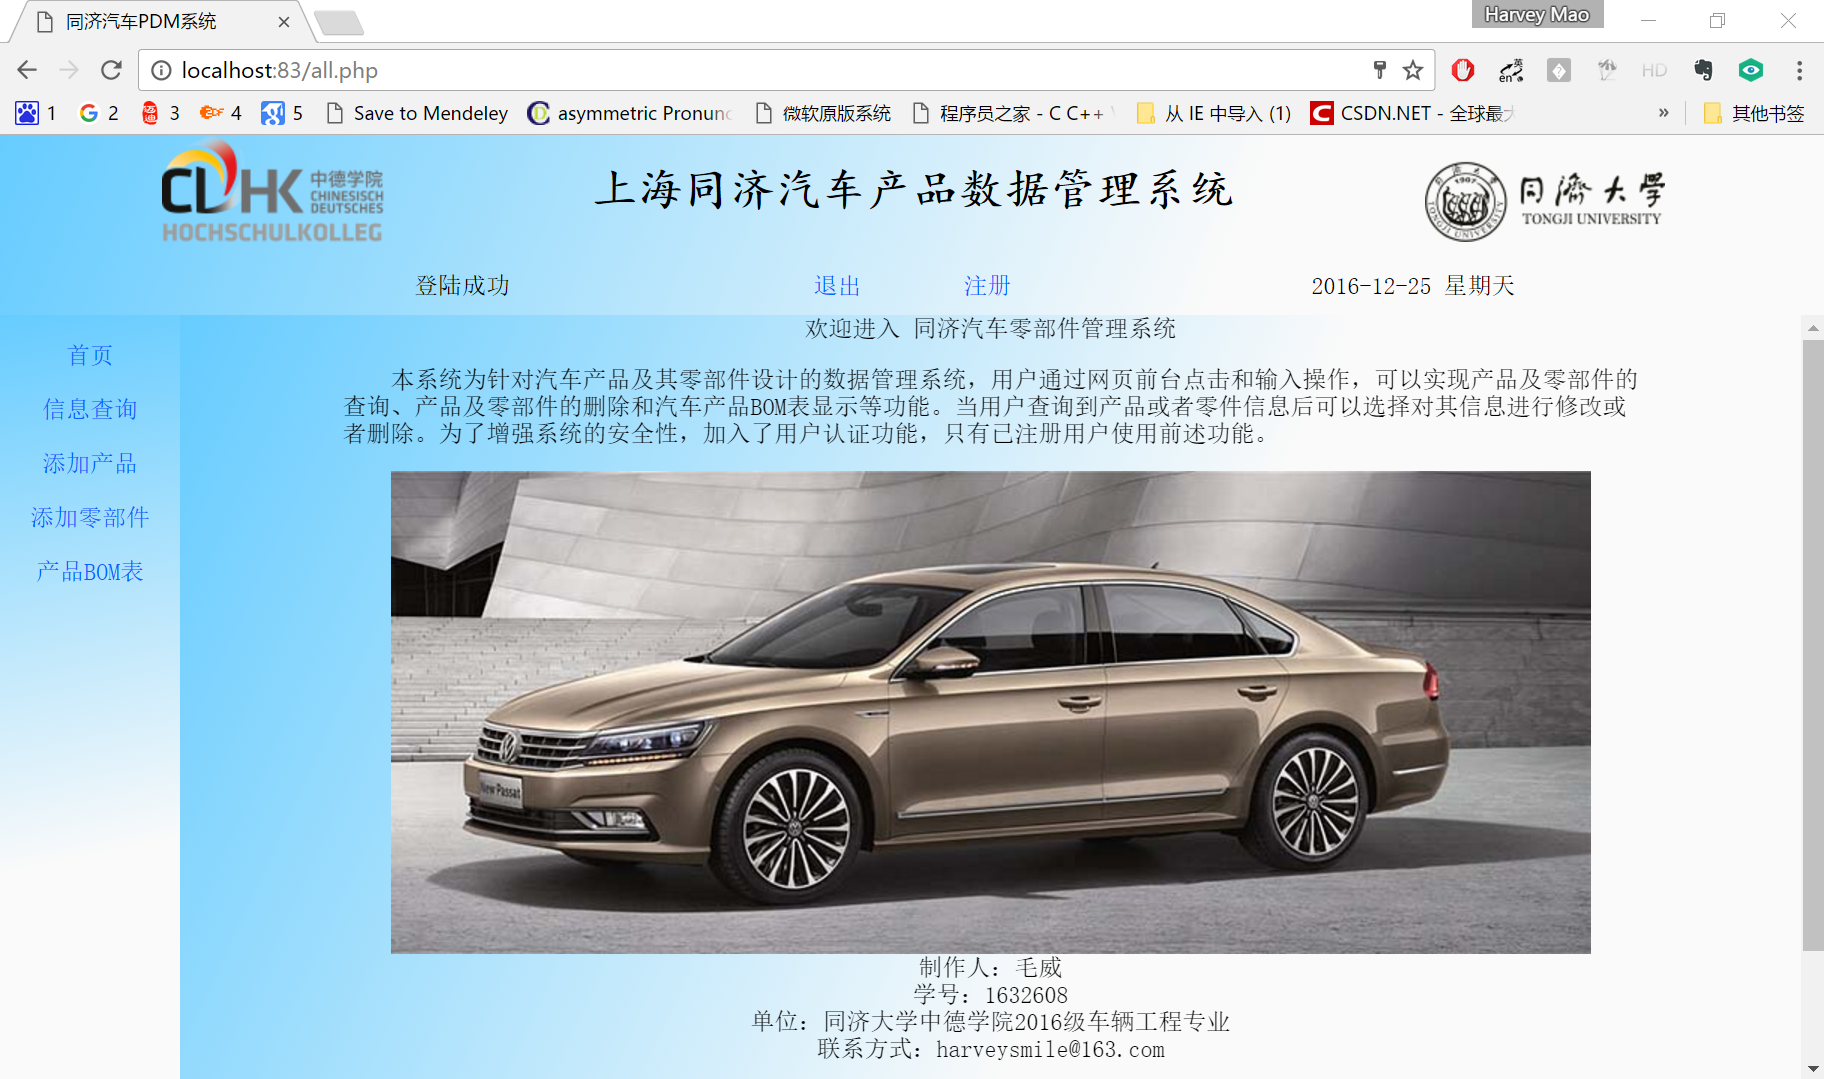
\includegraphics[width=0.9\linewidth]{figure/index}
\caption{汽车PDM主界面}
\label{fig:index1}
\end{figure}

\subsection{用户认证}
增加对用户的身份认证可以提高数据的安全性。非注册用户无法访问数据库完成各项功能。

在未登录网页的情况下点击主页\underline{信息查询、添加产品、添加零部件和产品BOM表},将弹出未登录对话框,如图\ref{fig:nologin}。
\begin{figure}[H]
\centering
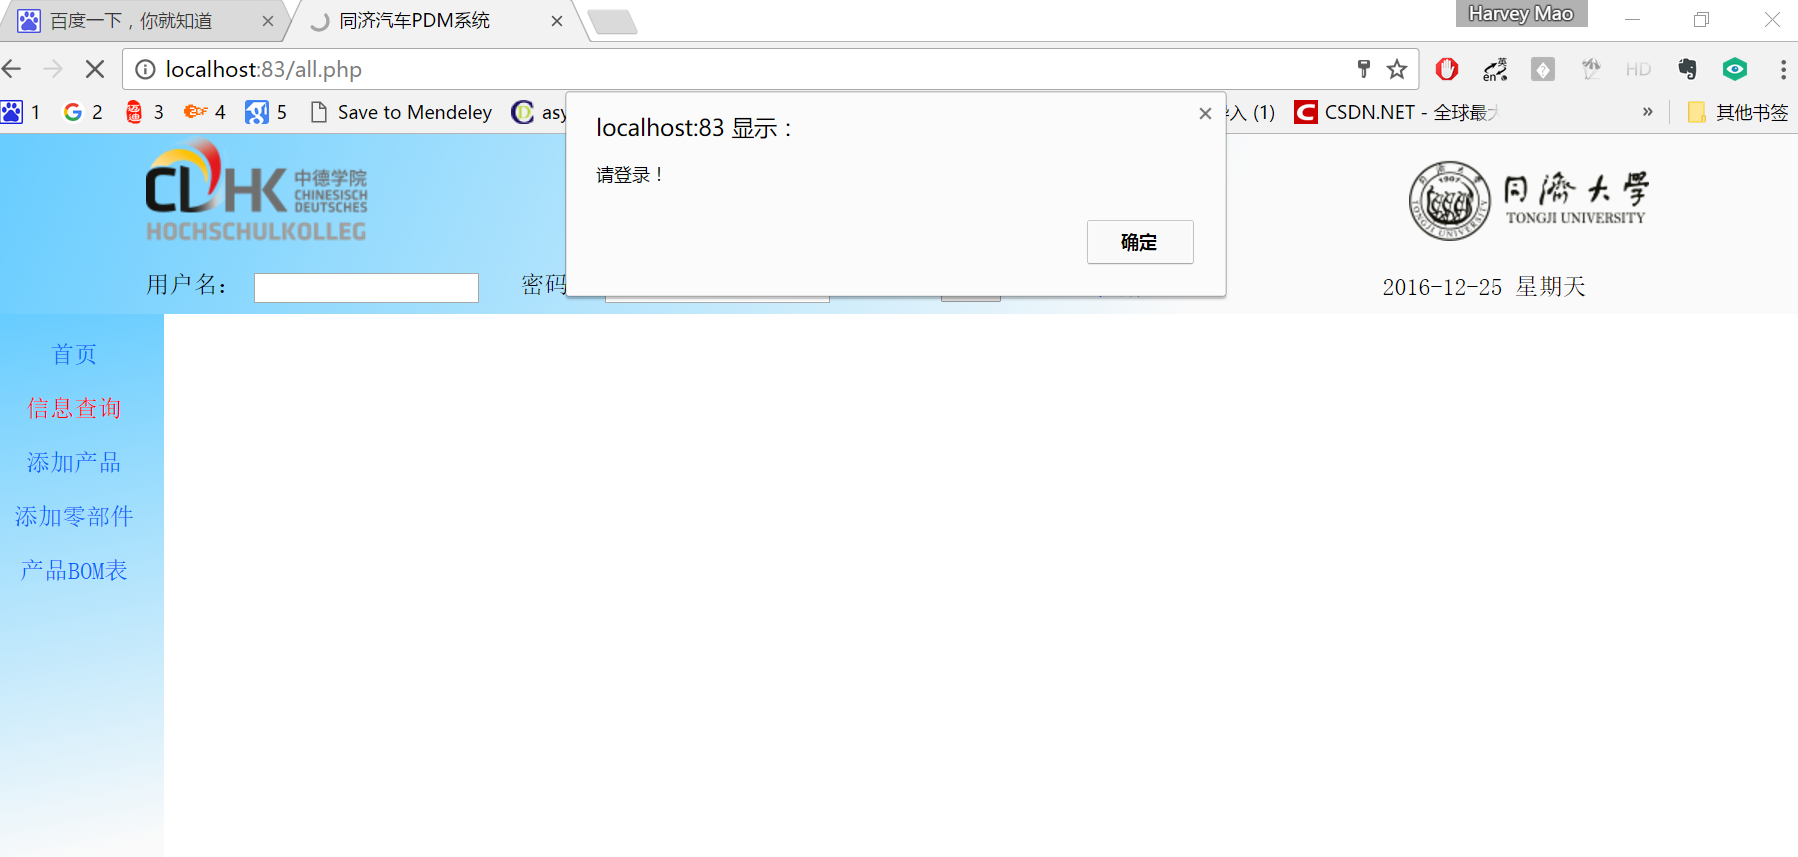
\includegraphics[width=0.9\linewidth]{figure/nologin}
\caption{未登录提醒}
\label{fig:nologin}
\end{figure}

点击\underline{注册},如图\ref{fig:reg}所示,输入用户名和密码,注意2次输入密码一致,否则注册失败。
\begin{figure}[H]
\centering
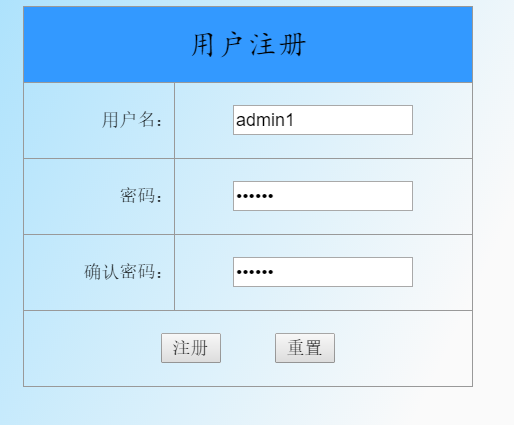
\includegraphics[width=0.8\linewidth]{figure/reg}
\caption{注册}
\label{fig:reg}
\end{figure}

输入用户名和密码,点击\underline{登陆},如图\ref{fig:printlogin}所示。
\begin{figure}[H]
\centering
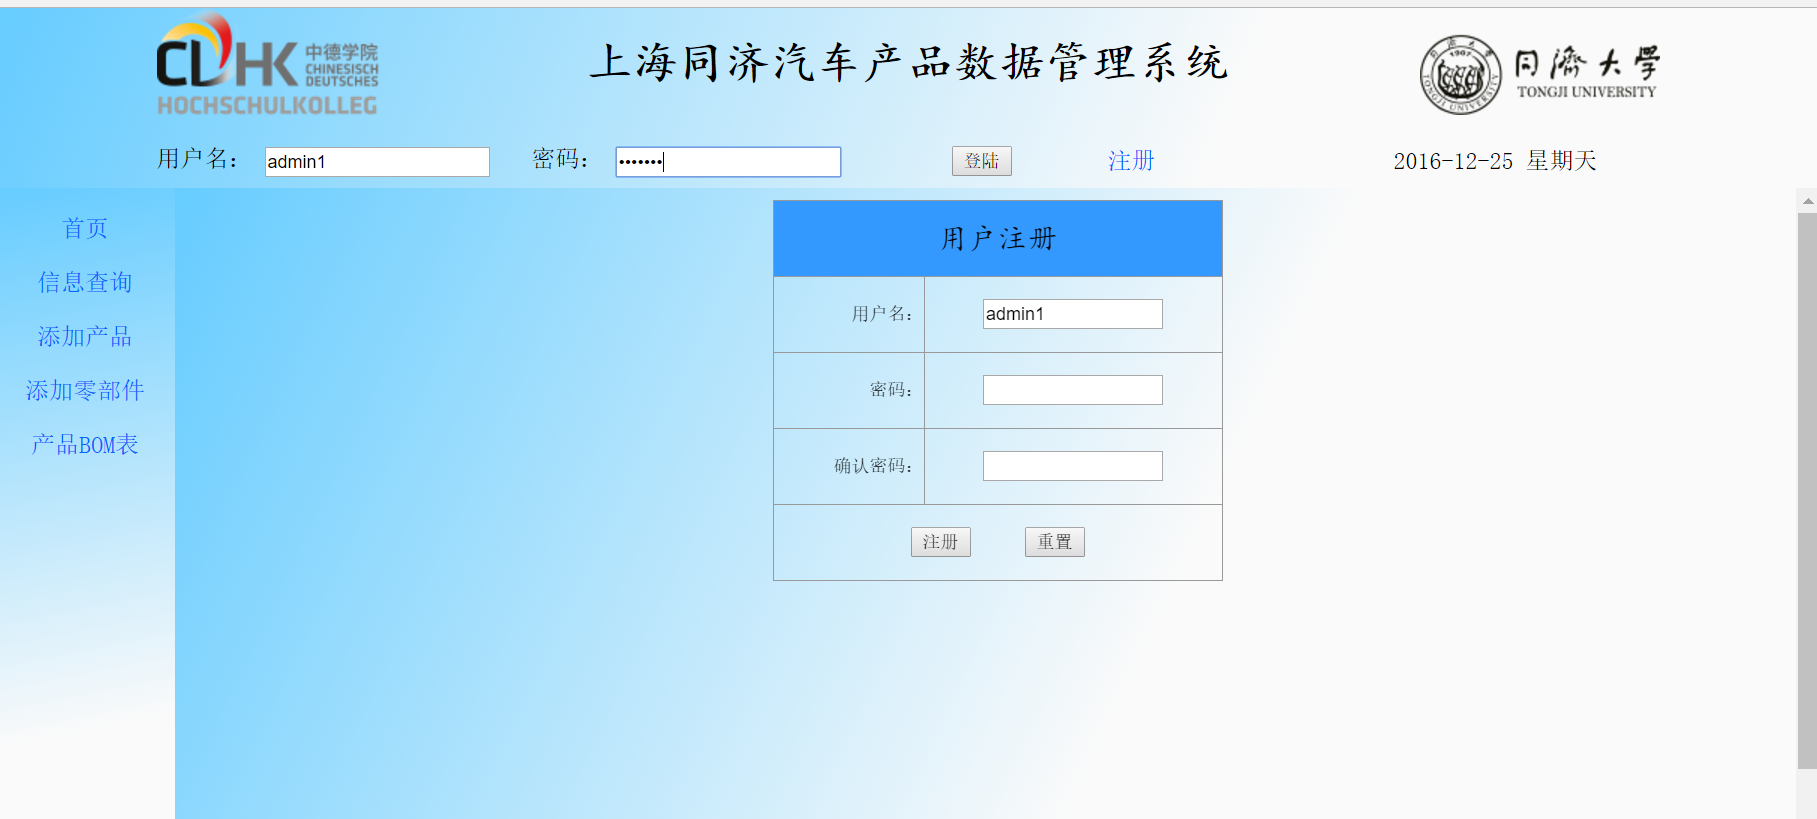
\includegraphics[width=0.7\linewidth]{figure/printlogin}
\caption{登陆}
\label{fig:printlogin}
\end{figure}

如果用户名和密码输入正确,则显示登陆成功,如图\ref{fig:sucesslogin}所示,否则登陆失败,如图\ref{fig:loslogin}所示.
\begin{figure}[H]
\centering
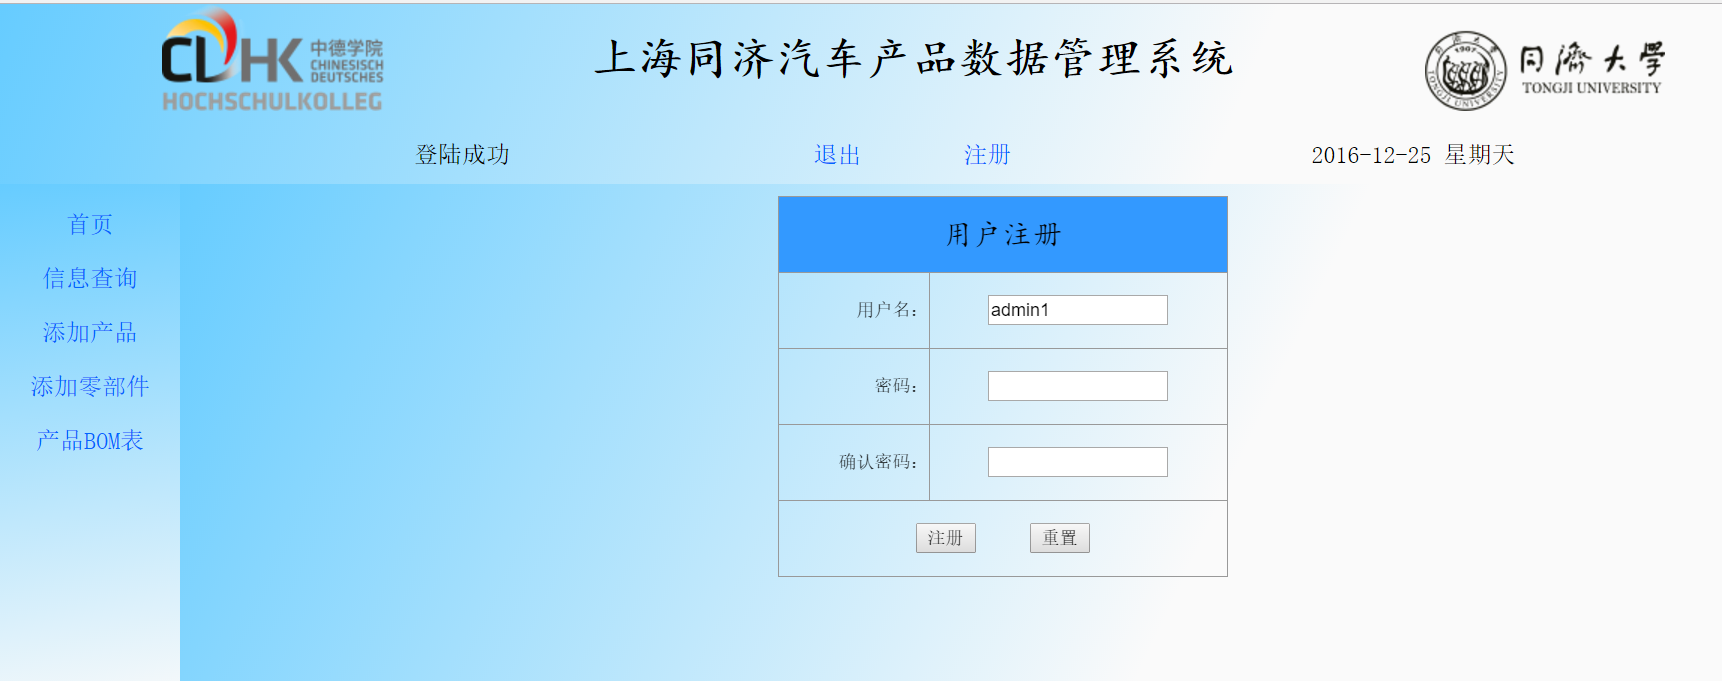
\includegraphics[width=0.9\linewidth]{figure/sucesslogin}
\caption{登陆成功}
\label{fig:sucesslogin}
\end{figure}

\begin{figure}[H]
\centering
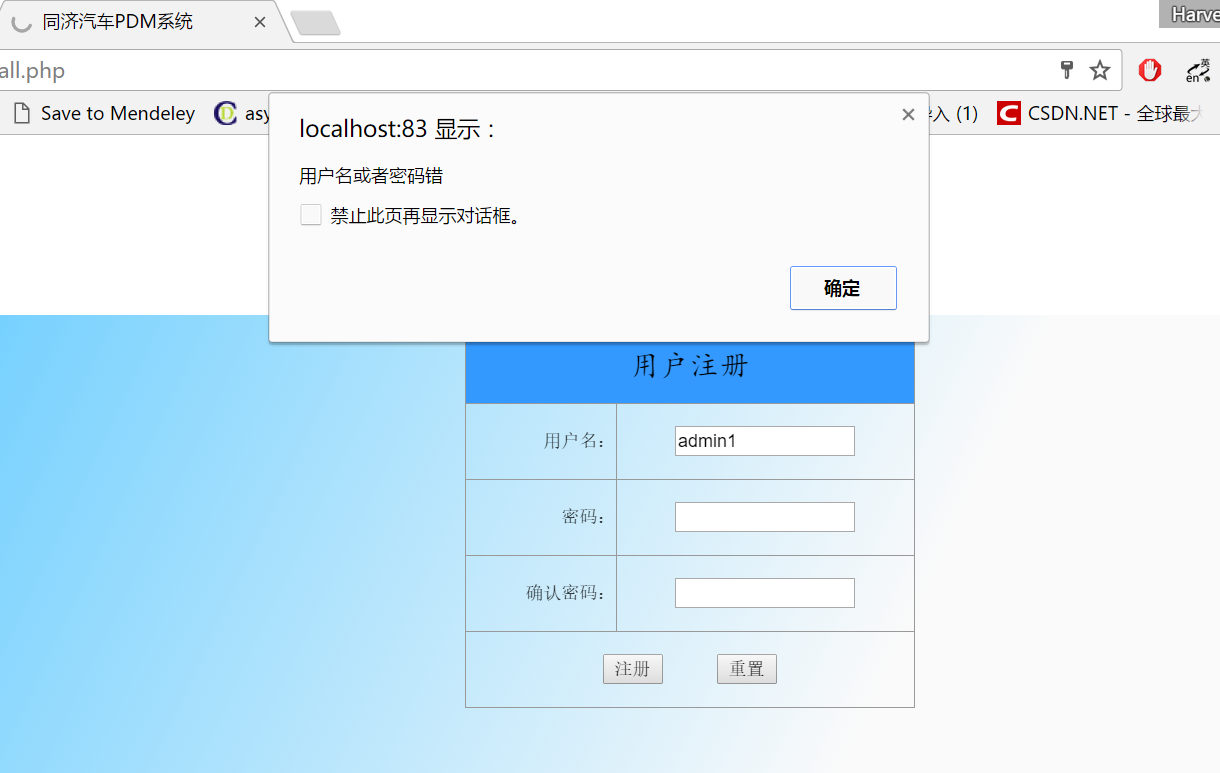
\includegraphics[width=0.9\linewidth]{figure/loslogin}
\caption{登陆失败弹框}
\label{fig:loslogin}
\end{figure}



\subsection{记录查询}

\subsubsection{简单查询模式}
点击主页\underline{信息查询},进入记录查询查询页面,如图\ref{fig:simplesearch}所示。简单查询模式支持某一字段(型号、名词、编号、制造商、产地)和价格做为查询条件,其中价格项目2个输入框分别为价格的最小最大值。三个输入框可以只输入1个或者输入2个或者全部输入,输入值之间构成``与''逻辑。
\begin{figure}[H]
\centering
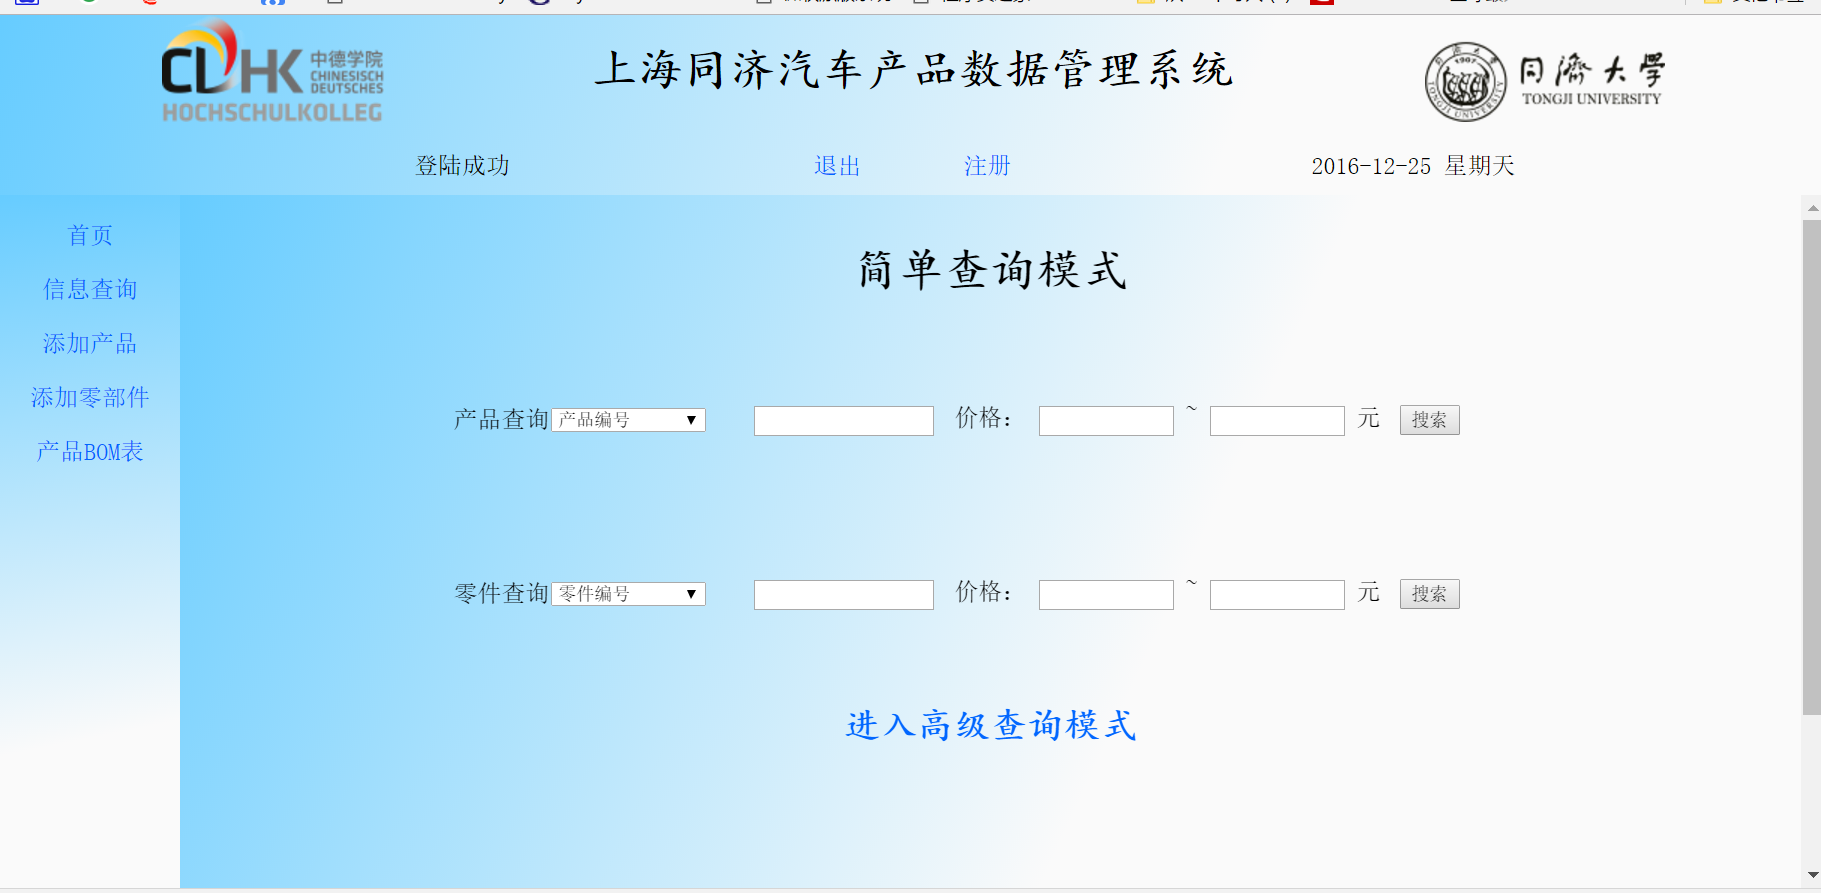
\includegraphics[width=0.8\linewidth]{figure/simplesearch}
\caption{信息查询页面}
\label{fig:simplesearch}
\end{figure}

在产品查询简单查询模式中输入如图\ref{fig:spsearch_prd_name}所示的条件,即查询产品名称为POLO的汽车产品,点击\underline{搜索},查询结果如图\ref{fig:spsearch_prd_name_result}所示。
\begin{figure}[H]
\centering
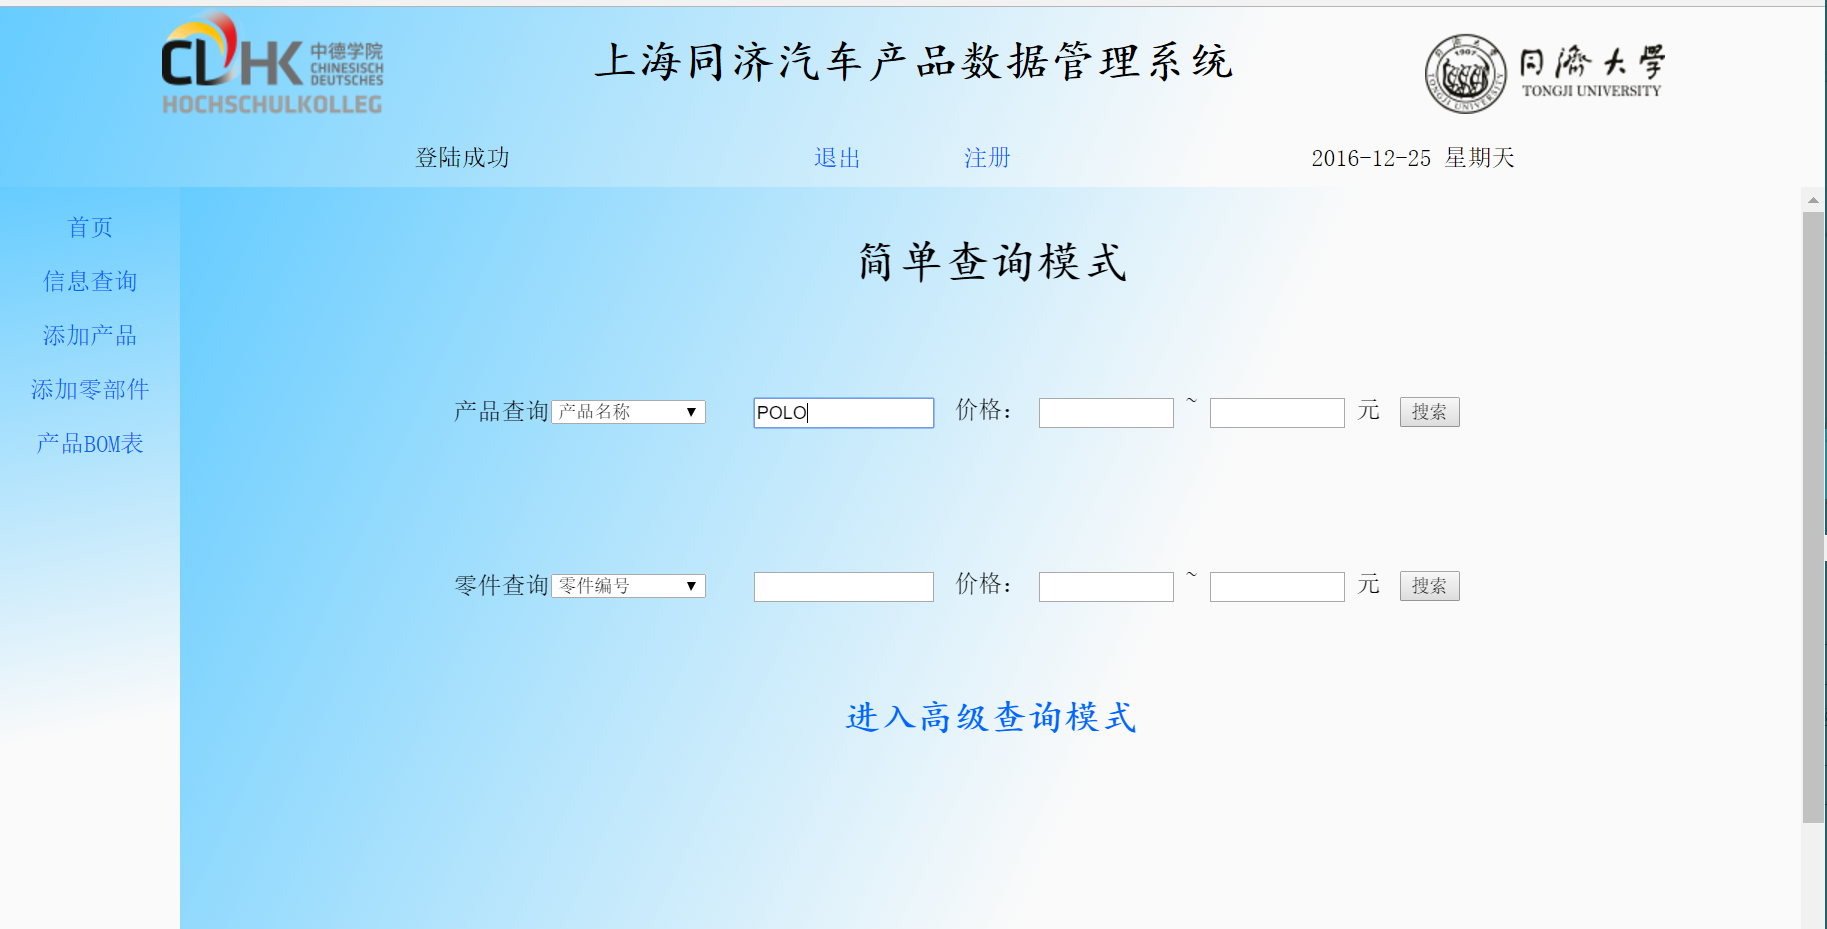
\includegraphics[width=0.9\linewidth]{figure/spsearch_prd_name}
\caption{简单搜索-产品名称}
\label{fig:spsearch_prd_name}
\end{figure}
\begin{figure}[H]
\centering
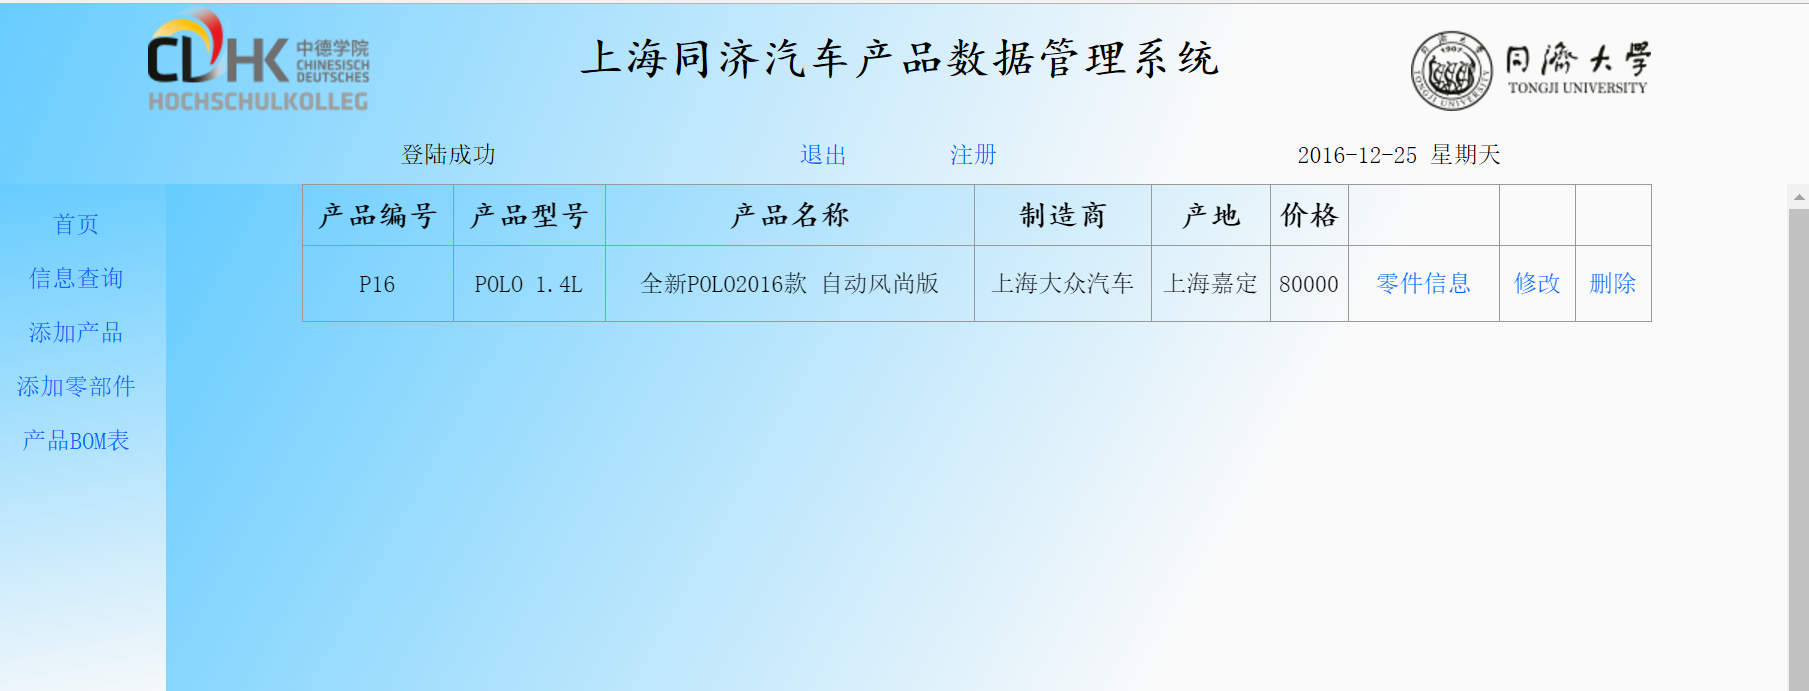
\includegraphics[width=0.9\linewidth]{figure/spsearch_prd_name_result}
\caption{简单搜索-产品名称-查询结果}
\label{fig:spsearch_prd_name_result}
\end{figure}

在零件查询简单查询模式中输入如图\ref{fig:spsea_part_area_price}所示的条件,即查询零件产地为上海并且价格低于1000元的汽车零件,点击\underline{搜索},查询结果如图\ref{fig:spsea_part_area_price_result}所示。
\begin{figure}[H]
\centering
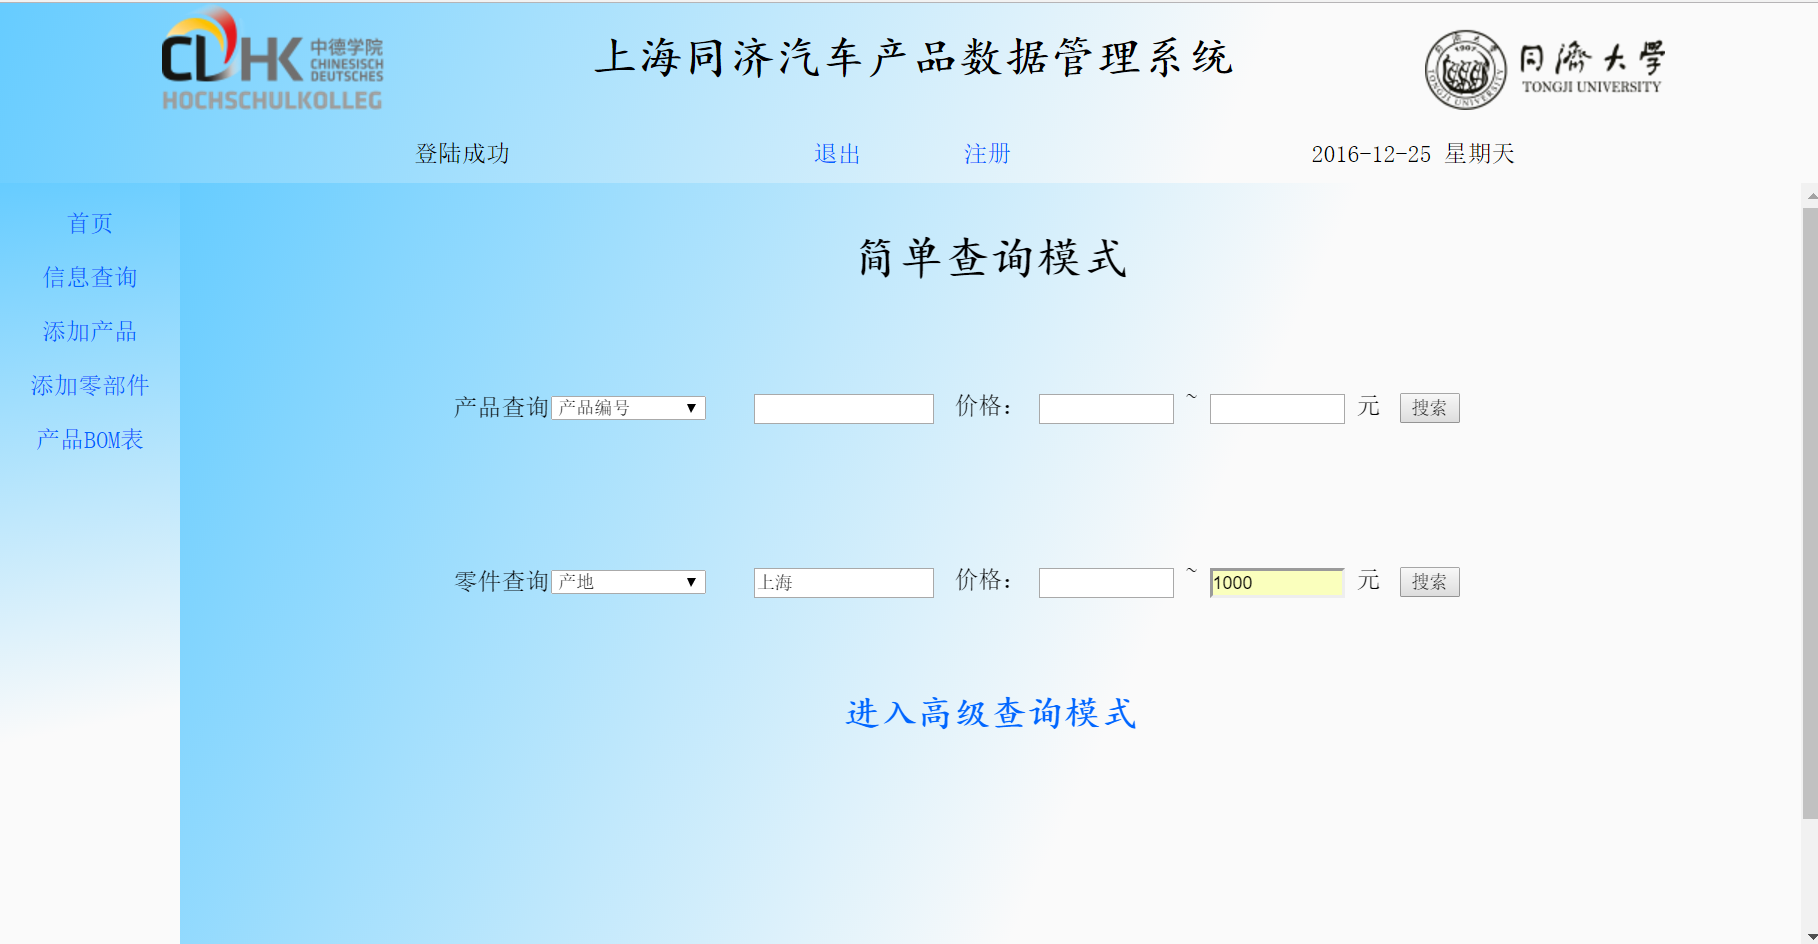
\includegraphics[width=0.9\linewidth]{figure/spsea_part_area_price}
\caption{简单查询-零件查询-产地/价格}
\label{fig:spsea_part_area_price}
\end{figure}

\begin{figure}[H]
\centering
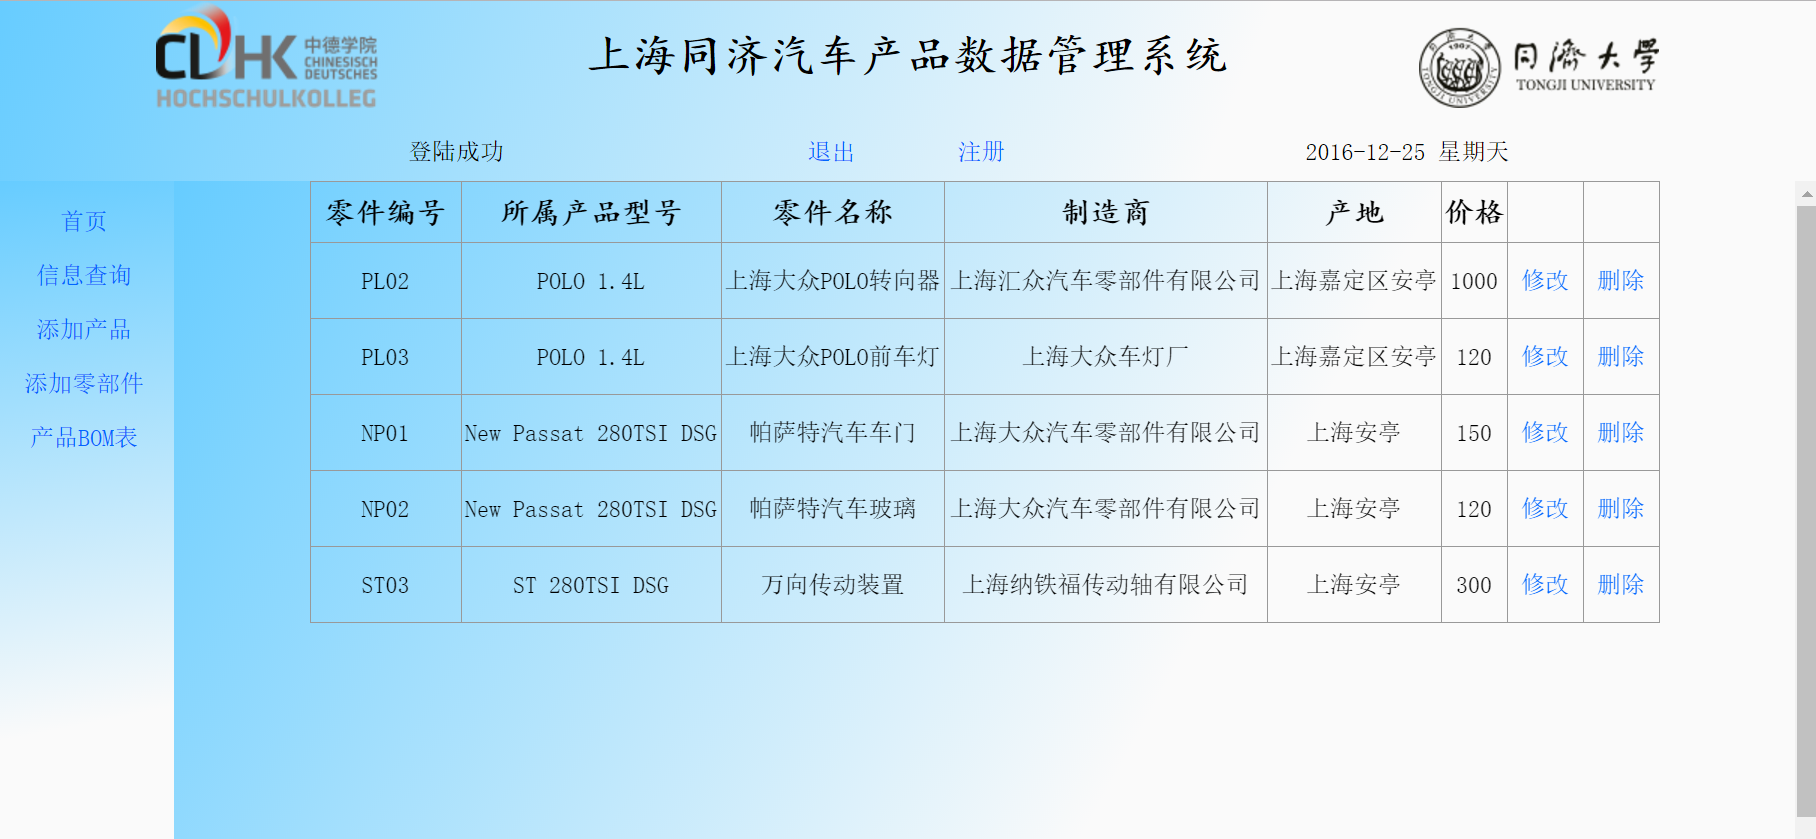
\includegraphics[width=0.9\linewidth]{figure/spsea_part_area_price_result}
\caption{简单查询-零件查询-产地/价格-查询结果}
\label{fig:spsea_part_area_price_result}
\end{figure}

本文设计的查询系统中各个文本字段值均采用模糊匹配方法,如图\ref{fig:spsea_part_area_price_result}所示,只要产地中包含图\ref{fig:spsea_part_area_price}中产地值\textbf{上海}的记录都视为满足条件。

对于价格字段中的输入框,如果只给左边框赋值$L$,则表示条件:价格$\ge L$。,如果只给右边框赋值$R$,则表示条件:价格$\le R$。如果左框赋值$L$,右框赋值$R$,则表示条件:$L \le$价格$\le R$。

如果输入的价格不为数字(如图\ref{fig:price_error}),则系统会弹出``价格必须为数字''的提示框(如图\ref{fig:price_error_alert})。
\begin{figure}[H]
\centering
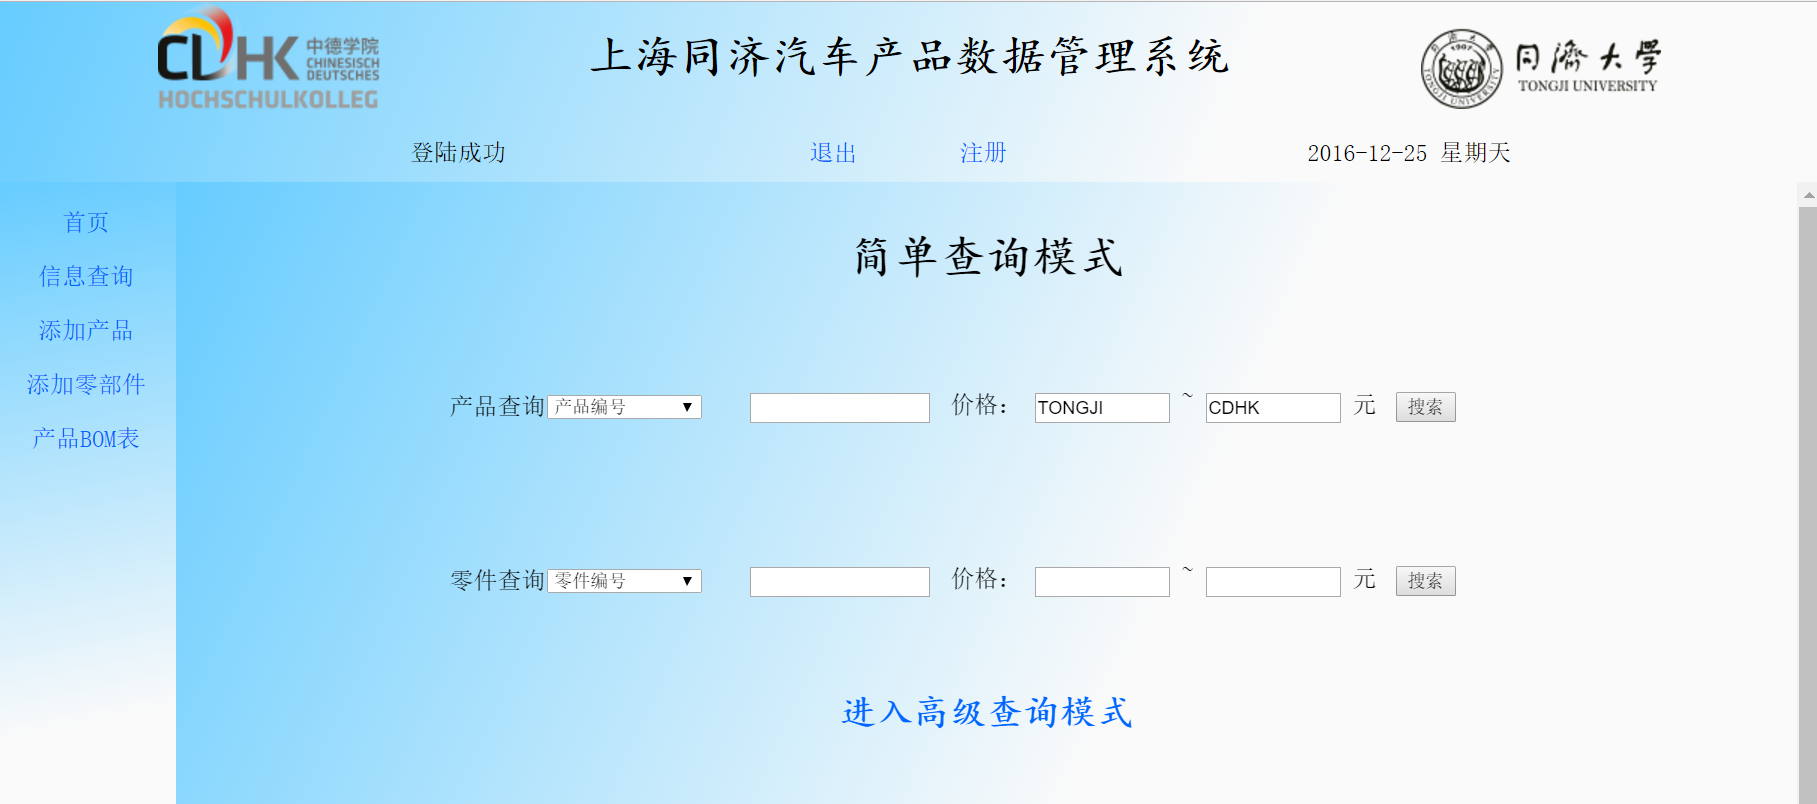
\includegraphics[width=0.9\linewidth]{figure/price_error}
\caption{错误价格格式}
\label{fig:price_error}
\end{figure}
\begin{figure}[H]
\centering
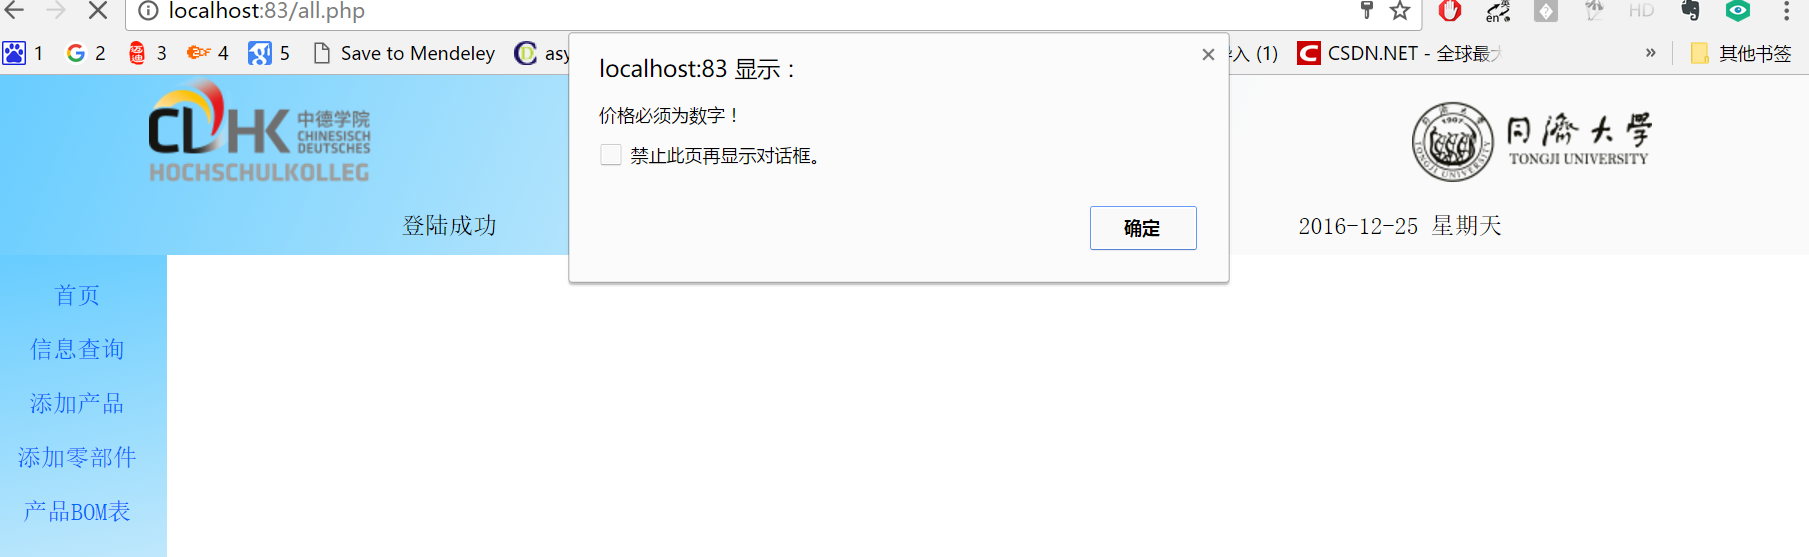
\includegraphics[width=0.9\linewidth]{figure/price_error_alert}
\caption{价格错误弹框}
\label{fig:price_error_alert}
\end{figure}

如果没有符合条件(如图\ref{fig:noreulscond})的结果,则系统会弹出``没有符合条件的记录''提示框(如图\ref{fig:noresult})。
\begin{figure}[H]
\centering
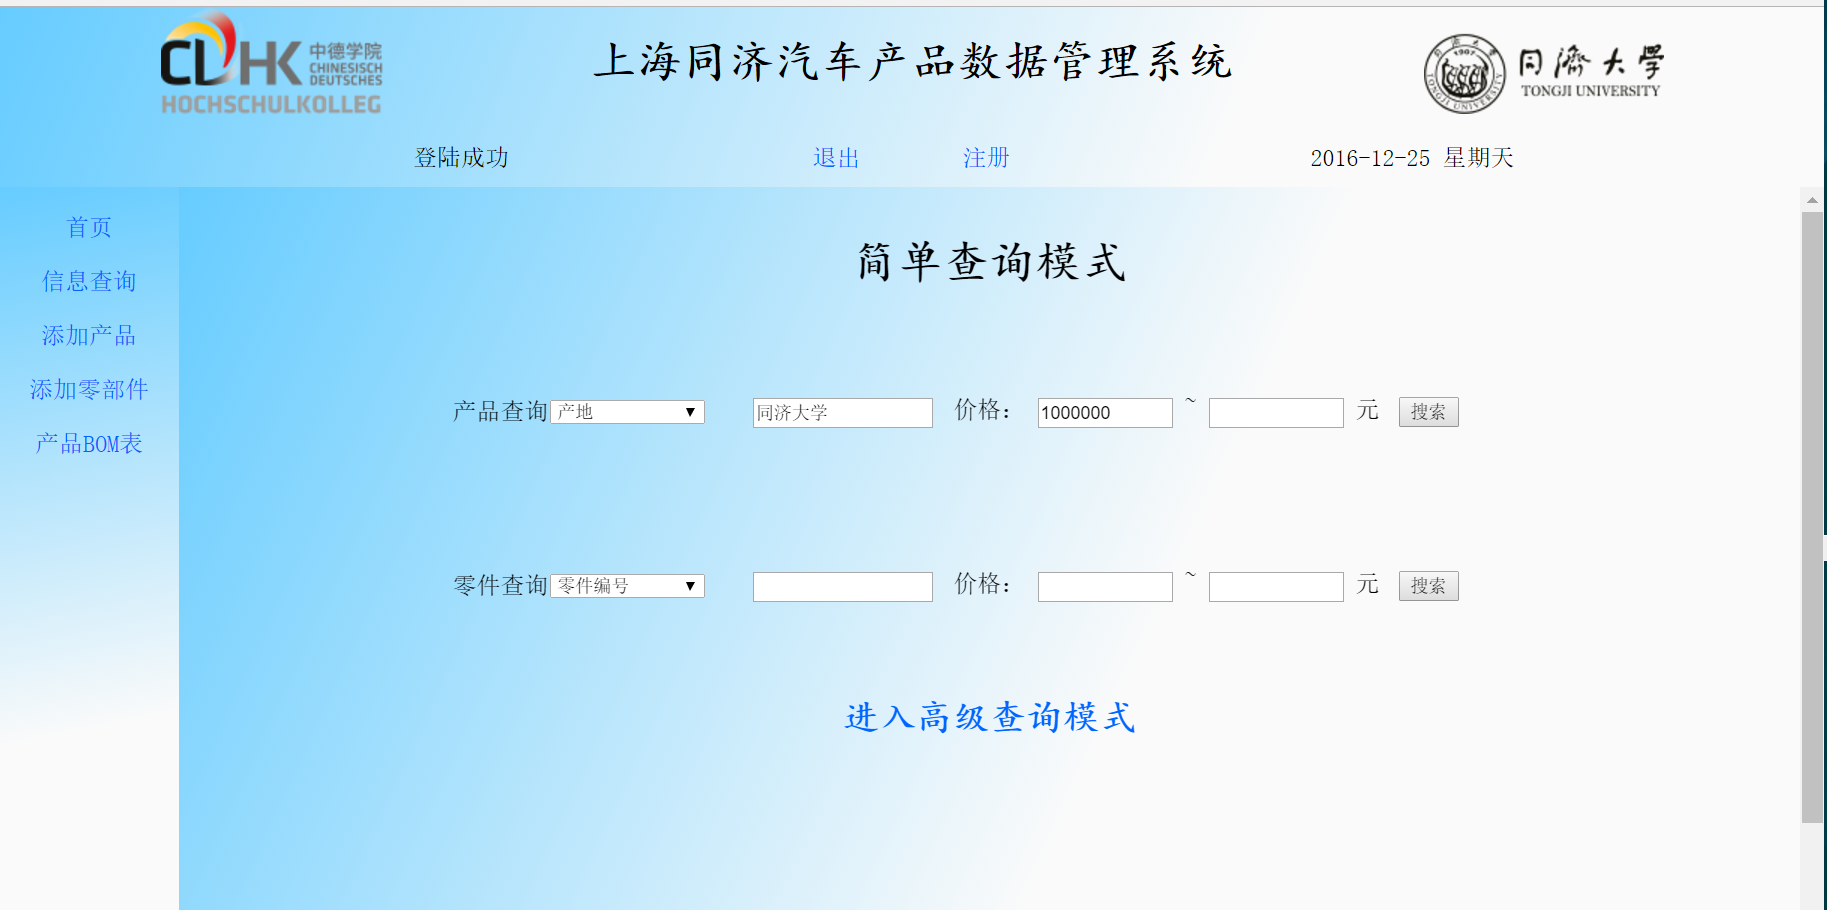
\includegraphics[width=0.9\linewidth]{figure/noreulscond}
\caption{无记录条件}
\label{fig:noreulscond}
\end{figure}

\begin{figure}[H]
\centering
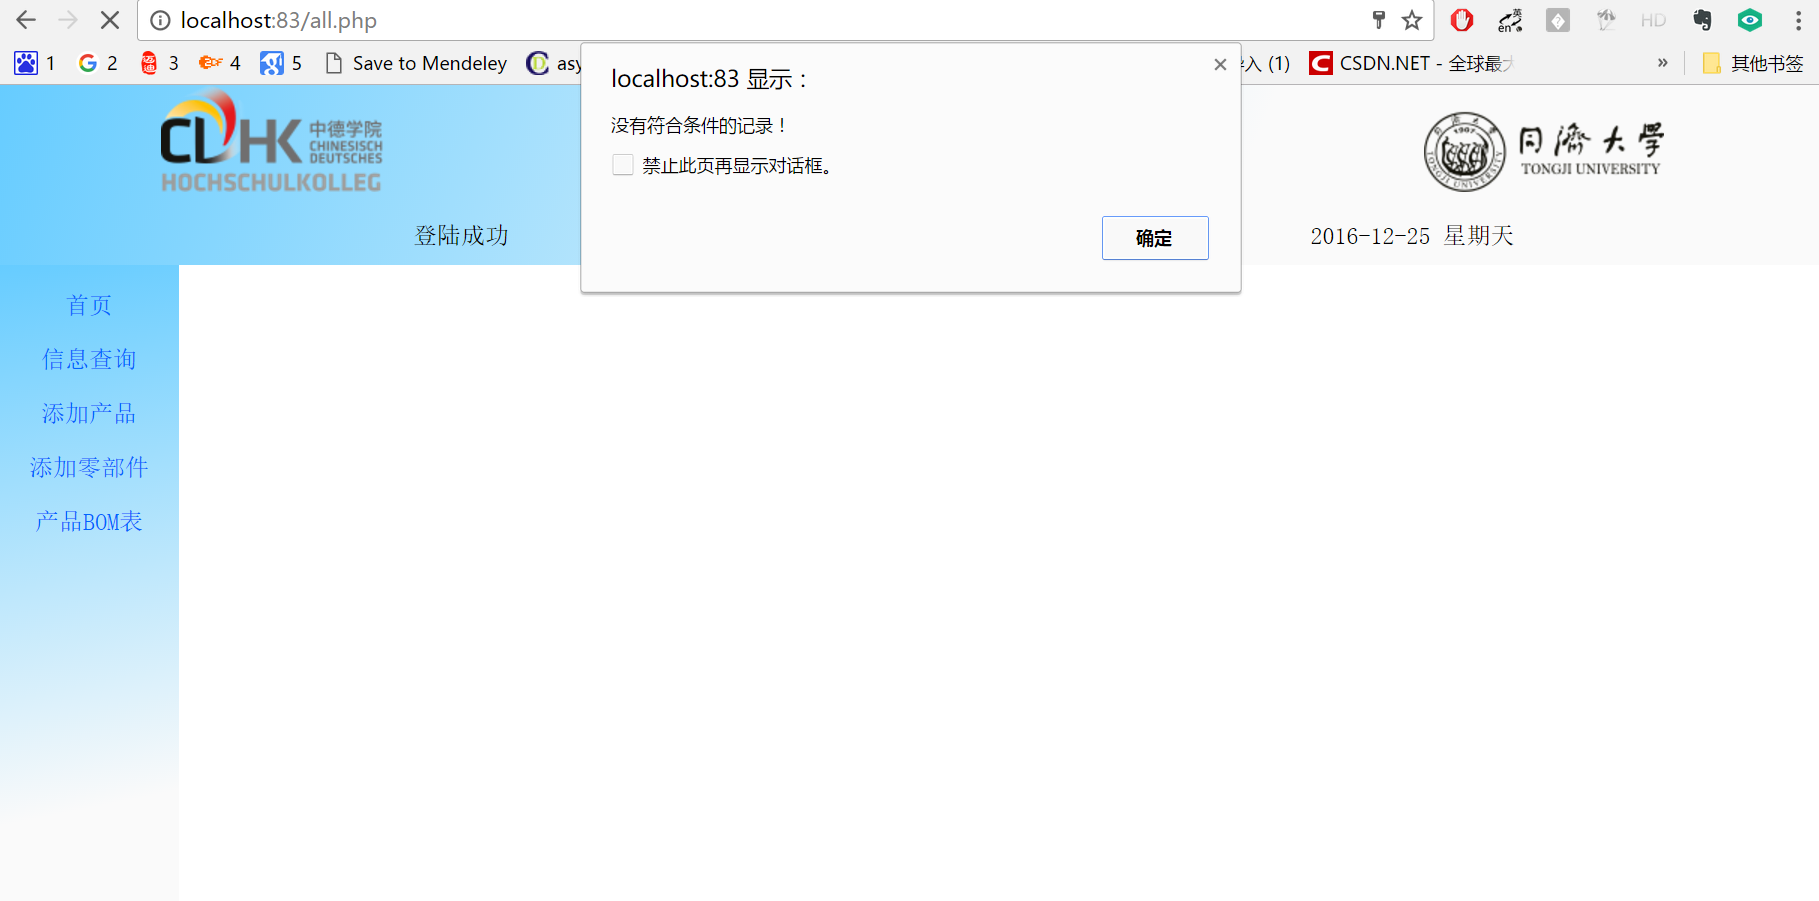
\includegraphics[width=0.9\linewidth]{figure/noresult}
\caption{``无符合条件记录''弹框}
\label{fig:noresult}
\end{figure}

\subsubsection{高级查询模式}
依次点击\underline{信息查询}$\to $\underline{进入高级查询模式}(如图\ref{fig:seniorSearInto_PxCook}),即可进入高级查询界面(如图\ref{fig:seniorSear})。
\begin{figure}[H]
\centering
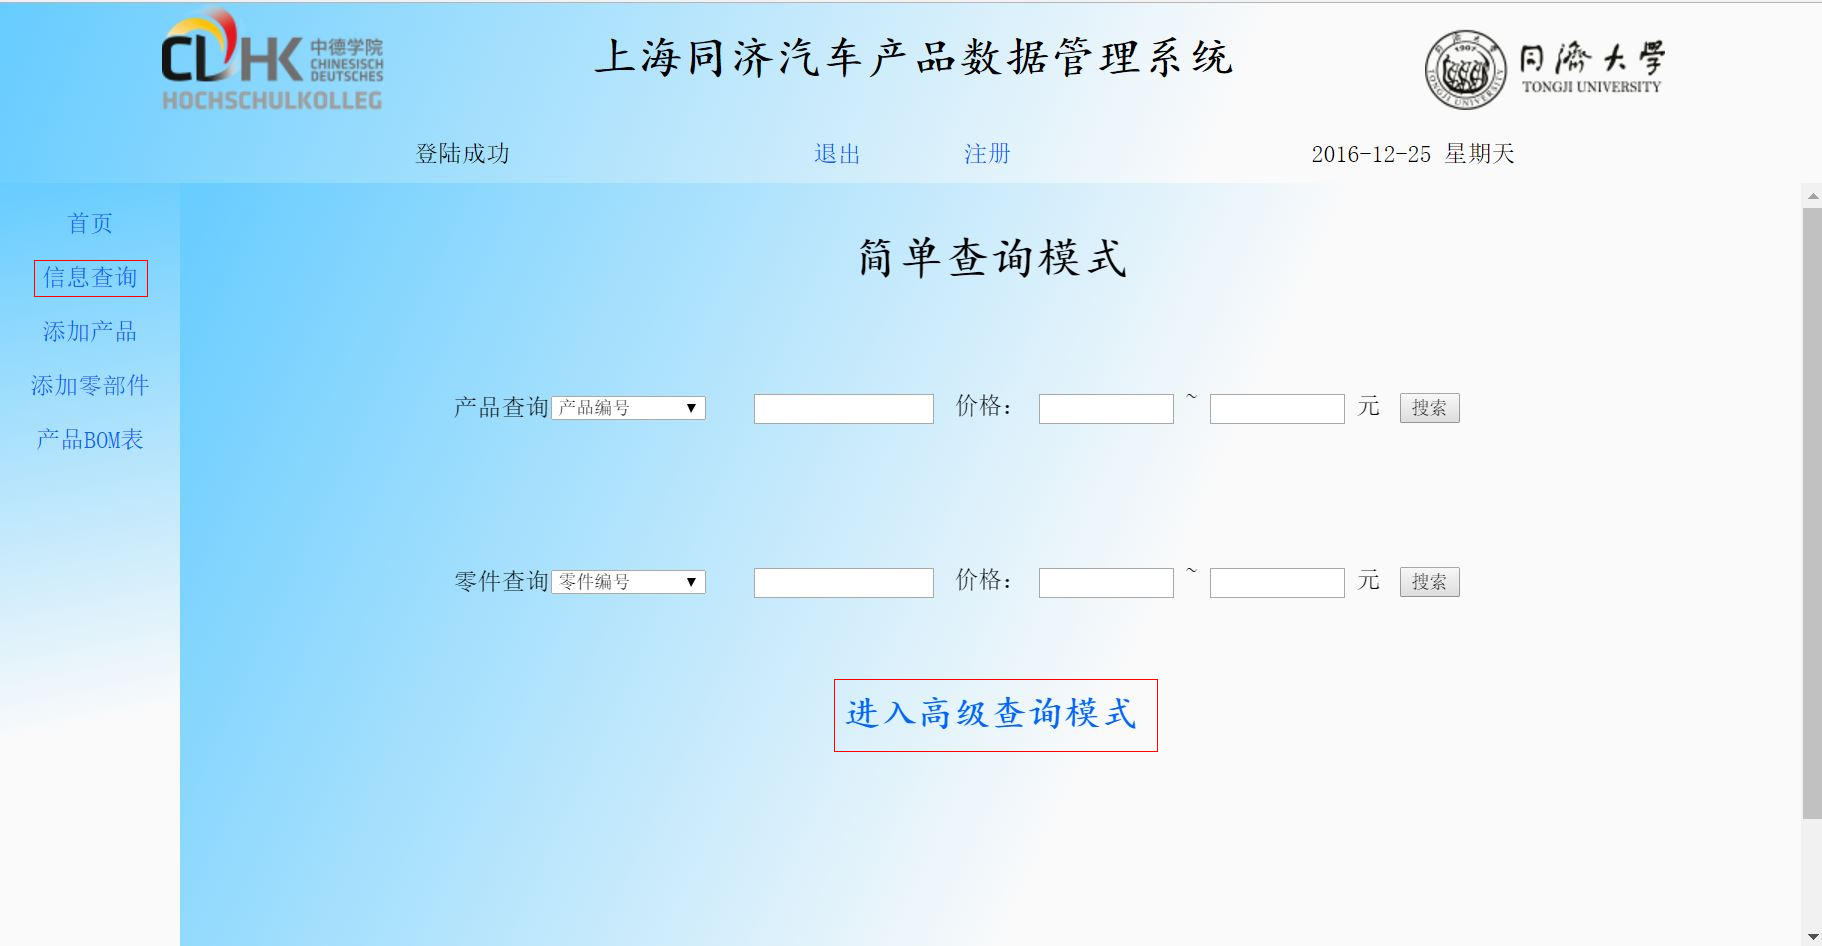
\includegraphics[width=0.9\linewidth]{figure/seniorSearInto_PxCook}
\caption{进入高级查询模式}
\label{fig:seniorSearInto_PxCook}
\end{figure}

\begin{figure}[H]
\centering
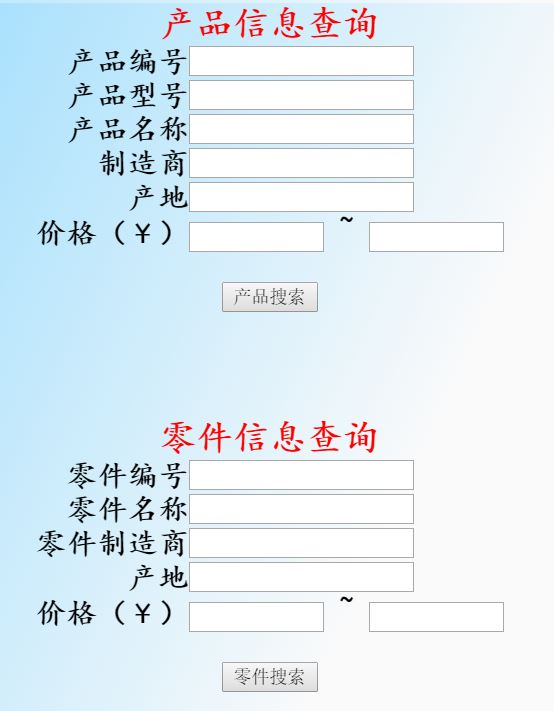
\includegraphics[width=0.7\linewidth]{figure/seniorSear}
\caption{高级查询模式}
\label{fig:seniorSear}
\end{figure}

高级查询模式支持所有字段任意组合成``与''逻辑的查询,可以给所有字段赋值,也可以只给部分字段赋值。

例如,在高级查询模式下,搜索条件如图\ref{fig:seniorPartSea}所示,即条件为产地含``武汉''字样、公司含``东风''字样、价格不超过200元,搜索结果如图\ref{fig:seniorPartRes}所示。

\begin{figure}[H]
\centering
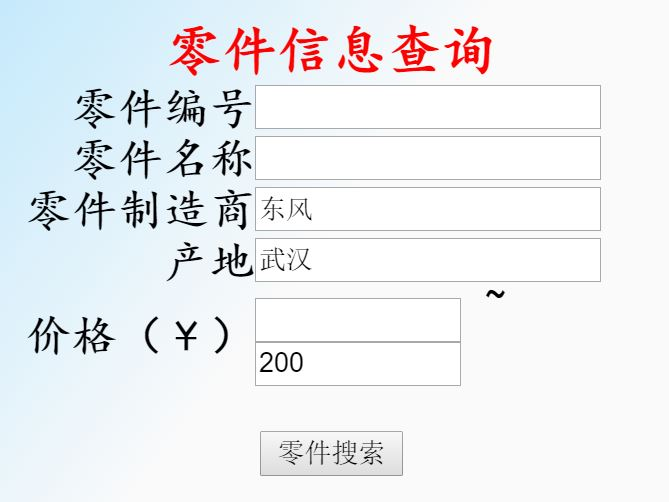
\includegraphics[width=0.7\linewidth]{figure/seniorPartSea}
\caption{高级零件查询示例}
\label{fig:seniorPartSea}
\end{figure}

\begin{figure}[H]
\centering

\includegraphics[width=0.9\linewidth]{figure/seniorPartRes}
\caption{高级零件查询示例结果}
\label{fig:seniorPartRes}
\end{figure}

和简单模式一样,各个字段依然为模糊搜索。如果输入的价格不为数字(如图\ref{fig:seniorNumError}),同样会有弹框(如图\ref{fig:seniorNumErrorAlert})。

\begin{figure}[H]
\centering
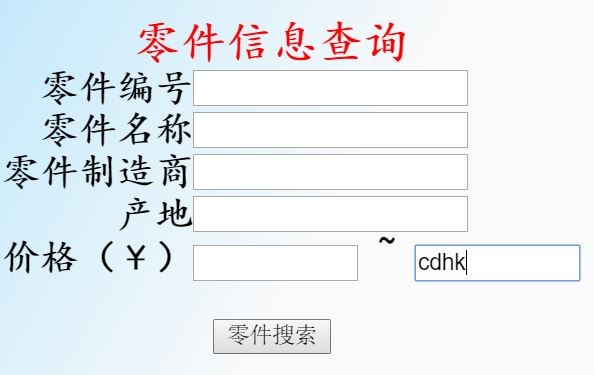
\includegraphics[width=0.7\linewidth]{figure/seniorNumError}
\caption{高级查询模式-价格格式错误}
\label{fig:seniorNumError}
\end{figure}

\begin{figure}[H]
\centering

\includegraphics[width=0.7\linewidth]{figure/seniorNumErrorAlert}
\caption{高级查询模式-价格错误弹窗}
\label{fig:seniorNumErrorAlert}
\end{figure}

\subsection{产品添加}
点击主页中\underline{添加产品},即可进入产品添加页面(如图\ref{fig:prod_add_index})。在页面中输入产品编号	 、产品型号、产品名称、产品制造商、产品产地和产品价格,所有项目为必填项,否则会弹框提醒(如图\ref{fig:error_noComplete}和\ref{fig:error_noComplete_alert})。此外价格必须为数字,否则也会报错(如图\ref{fig:prod_add_price_error}和\ref{fig:prod_add_price_error_alert})。
\begin{figure}[H]
\centering
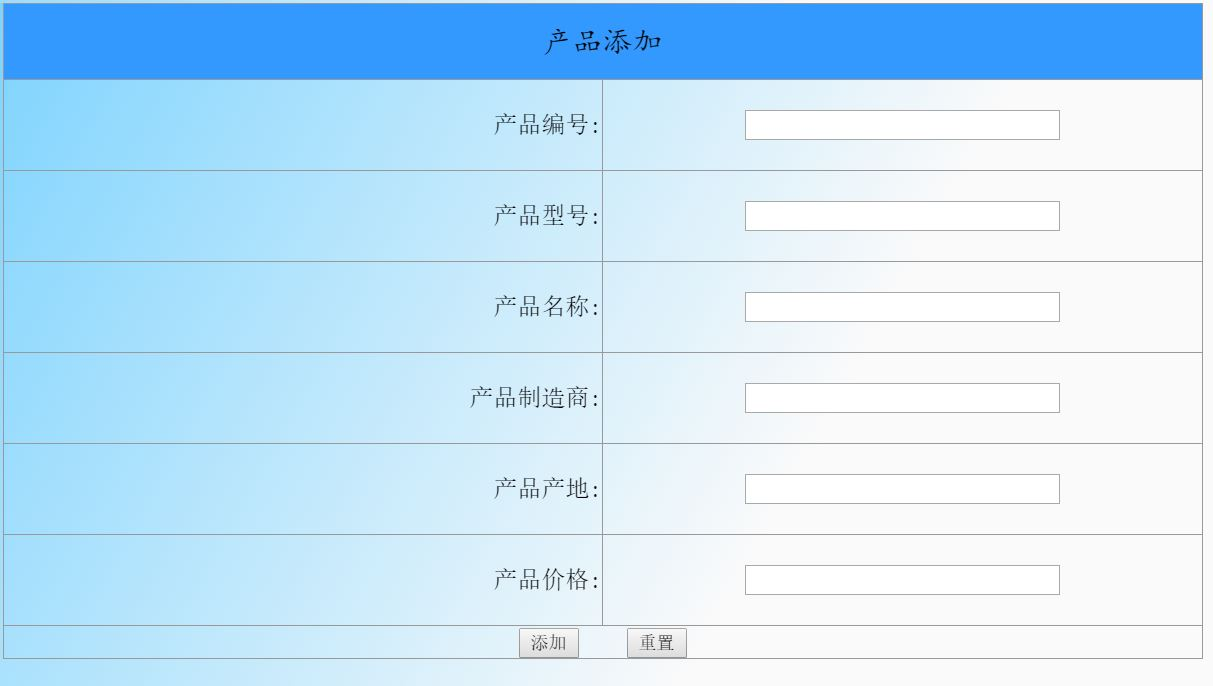
\includegraphics[width=0.8\linewidth]{figure/prod_add_index}
\caption{产品添加页面}
\label{fig:prod_add_index}
\end{figure}

\begin{figure}[H]
\centering
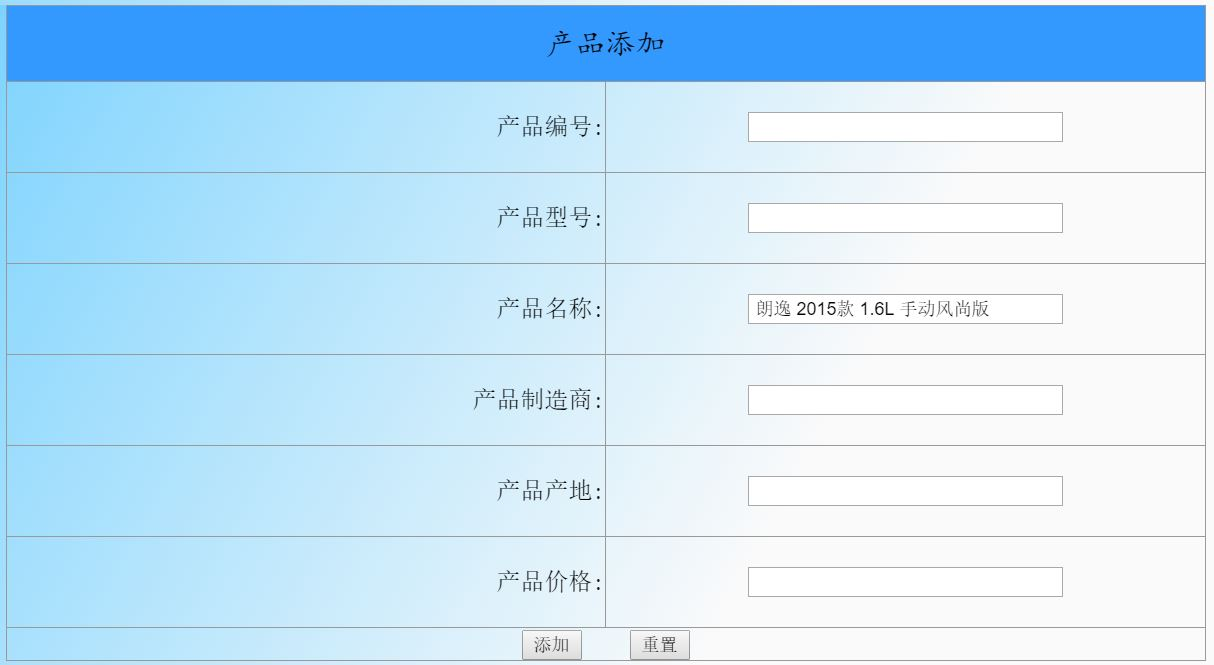
\includegraphics[width=0.8\linewidth]{figure/error_noComplete}
\caption{产品信息不完整}
\label{fig:error_noComplete}
\end{figure}

\begin{figure}[H]
\centering

\includegraphics[width=0.8\linewidth]{figure/error_noComplete_alert}
\caption{产品信息不完整提示}
\label{fig:error_noComplete_alert}
\end{figure}

\begin{figure}[H]
\centering
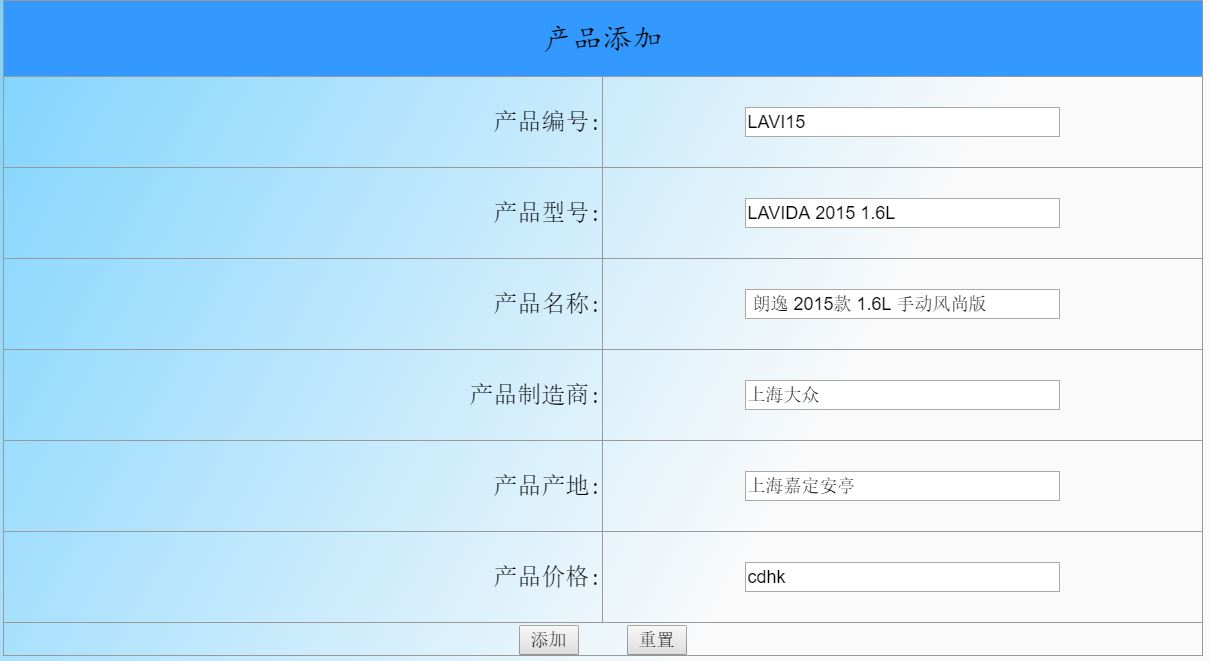
\includegraphics[width=0.8\linewidth]{figure/prod_add_price_error}
\caption{产品价格错误}
\label{fig:prod_add_price_error}
\end{figure}

\begin{figure}[H]
\centering
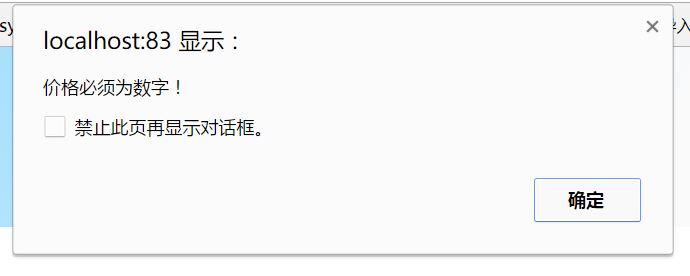
\includegraphics[width=0.8\linewidth]{figure/prod_add_price_error_alert}
\caption{产品价格错误提示}
\label{fig:prod_add_price_error_alert}
\end{figure}

在产品添加栏输入网址信息且保证价格为数字(如图\ref{fig:prod_add_sucess_inf}),点击\underline{添加},弹出添加成功提示(如图\ref{fig:prod_add_sucess})。
\begin{figure}[H]
\centering
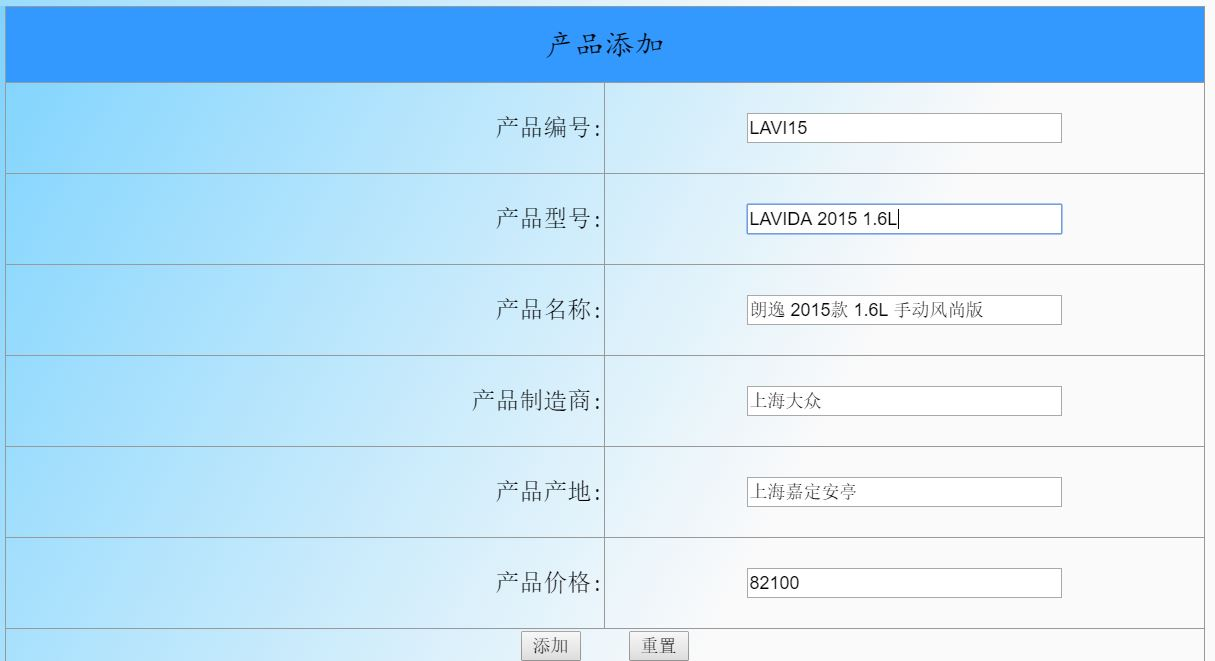
\includegraphics[width=0.8\linewidth]{figure/prod_add_sucess_inf}
\caption{产品信息完整且价格格式正确}
\label{fig:prod_add_sucess_inf}
\end{figure}
\begin{figure}[H]
\centering
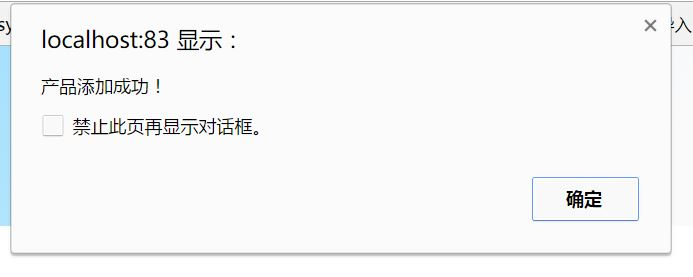
\includegraphics[width=0.8\linewidth]{figure/prod_add_sucess}
\caption{产品添加成功}
\label{fig:prod_add_sucess}
\end{figure}

\subsection{零部件添加}
点击主页中\underline{添加零部件},即可进入零部件添加页面,如图\ref{fig:part_add_index}。零部件所属产品型号是已经添加了的产品,拉下拉菜单可选择相应所属产品的型号,如选择New Passat 280TSI DSG。在这个页面中可添加零部件编号、零部件名称、零部件制造商、零部件产地和零部件价格,和产品添加一页面一样,这些项目都是必填字段,否则会弹出提醒``属性值不能为空'',其中价格必须为数字,否则也会弹框提醒。
\begin{figure}[H]
\centering
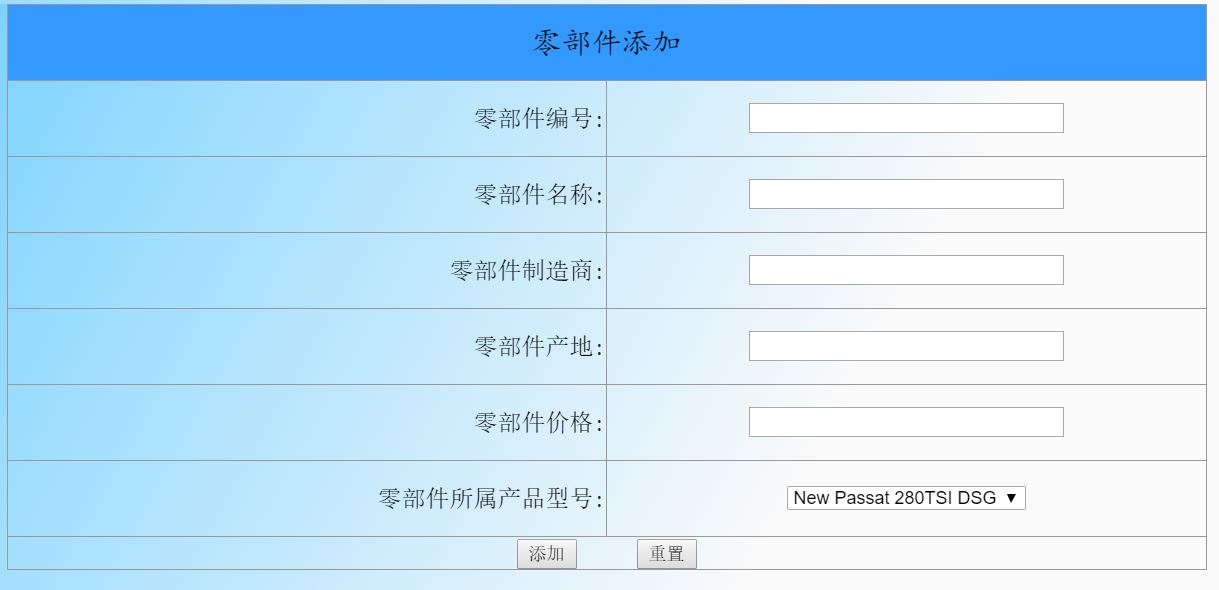
\includegraphics[width=0.9\linewidth]{figure/part_add_index}
\caption{零部件添加页面}
\label{fig:part_add_index}
\end{figure}

比如在页面中输入如图\ref{fig:part_add_inf}所示的零件信息,并且在下拉菜单中选择对应的产品型号。点击\underline{添加}按钮,即弹出添加成功提示d对话框\ref{fig:par_add_success},点击\underline{确认},回到零件添加页面\ref{fig:part_index1}。

\begin{figure}[H]
\centering
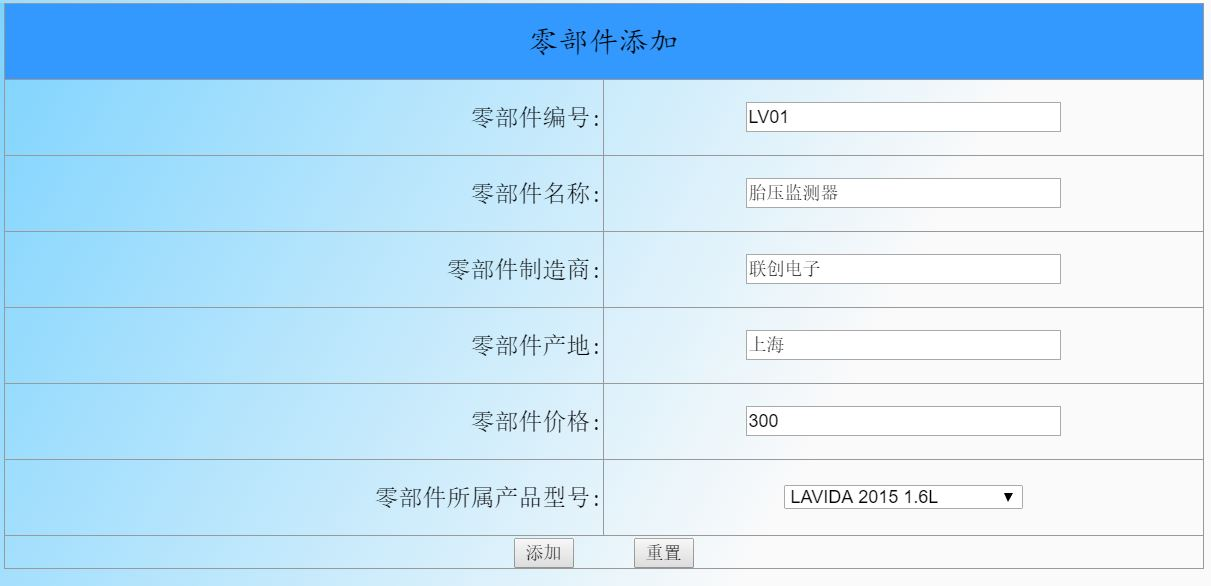
\includegraphics[width=0.8\linewidth]{figure/part_add_inf}
\caption{添加零部件}
\label{fig:part_add_inf}
\end{figure}

\begin{figure}[H]
\centering

\includegraphics[width=0.9\linewidth]{figure/par_add_success}
\caption{零部件添加成功}
\label{fig:par_add_success}
\end{figure}

\begin{figure}[H]
\centering
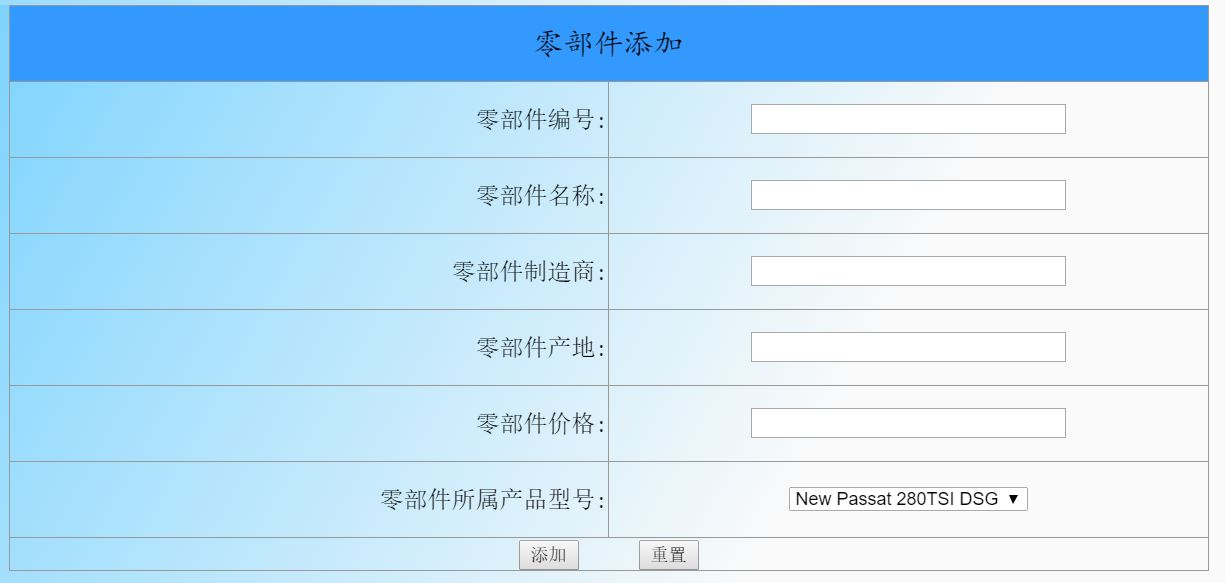
\includegraphics[width=0.8\linewidth]{figure/part_index1}
\caption{零件添加页面}
\label{fig:part_index1}
\end{figure}

\subsection{附属零件信息显示}
在产品查询页面中,输入查询条件,完成查询,将在界面上显示了产品查询结果,如图\ref{fig:spsearch_prd_name_result}所示。产品结果以表格形式给出,每一行代表一个产品记录,点击每一行后的\underline{零件信息},即可显示零件信息,图\ref{fig:POLO_part_infDetail}为汽车产品POLO 1.4L在MySQL数据库中的附属零件信息。
\begin{figure}[H]
\centering
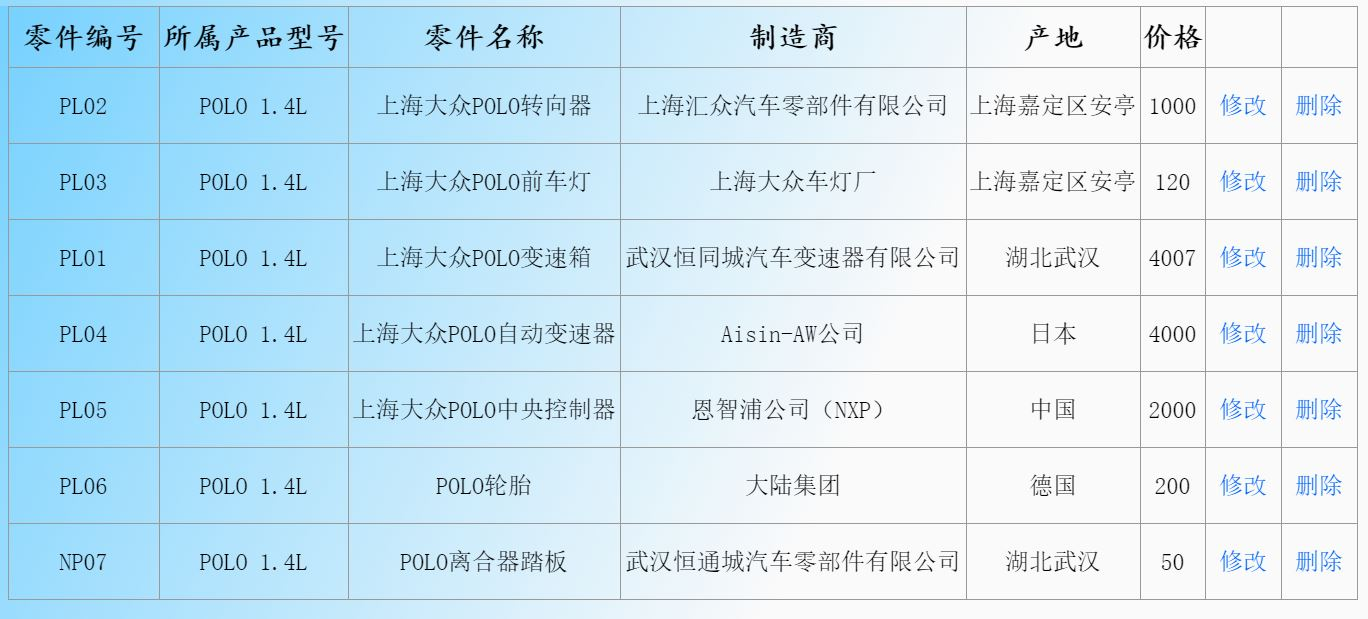
\includegraphics[width=0.8\linewidth]{figure/POLO_part_infDetail}
\caption{POLO 1.4L附属零件信息}
\label{fig:POLO_part_infDetail}
\end{figure}

在``删除后的产品记录''中也\underline{零件信息}链接;通过BOM表产品链接中也可以进入对应产品记录页面,该页面中同样也有\underline{零件信息}链接。
\subsection{记录删除}
本系统支持产品记录和零件的删除,系统在数据库建模时,将汽车产品和零部件的关系定义为``一对多''的关系,且支持外键约束,\textbf{即当用户将汽车产品删除后,对应的零件将全部自动删除},这一点用户需要注意。

在产品查询页面中,输入查询条件产品型号:LAVIDA 2016 1.6L,完成查询,将在界面上显示了产品查询结果,如图\ref{fig:LV16_prd_inf}所示。产品结果以表格形式给出,每一行代表一个产品记录,点击\underline{零件信息},LAVIDA 2016 1.6L的零件信息如图\ref{fig:LV16_prd_part_inf}所示,
\begin{figure}[H]
\centering
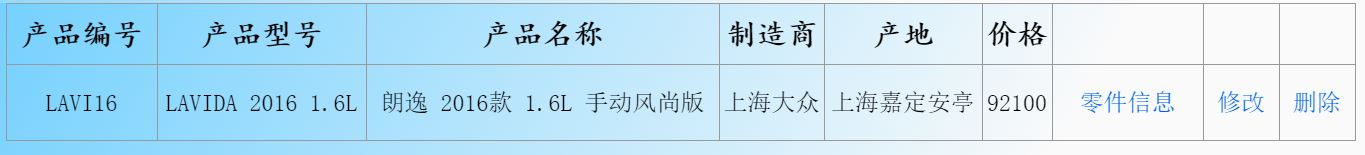
\includegraphics[width=0.9\linewidth]{figure/LV16_prd_inf}
\caption{LAVIDA 2016 1.6L}
\label{fig:LV16_prd_inf}
\end{figure}

\begin{figure}[H]
\centering
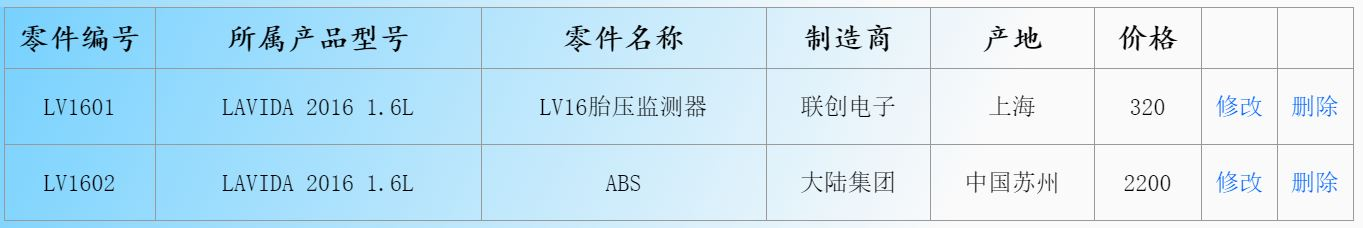
\includegraphics[width=0.9\linewidth]{figure/LV16_prd_part_inf}
\caption{LAVIDA 2016 1.6L 零件信息}
\label{fig:LV16_prd_part_inf}
\end{figure}


点击LAVIDA 2016 1.6L所在行后的\underline{删除}链接,即可删除汽车产品。同时其附属零件也将自动删除。为了防止误删,在点击删除后会弹出提醒对话框如图\ref{fig:prd_delete_alert},点击\underline{确认},将弹出删除成功对话框如图\ref{fig:prd_delete_success_alert},接着点击\underline{确认},即可显示删除之后,数据库中的产品记录如图\ref{fig:prd_deleteLV16}。其附属零件也将删除。
\begin{figure}[H]
\centering
\includegraphics[width=0.8\linewidth]{figure/prd_delete_alert}
\caption{产品删除提醒对话框}
\label{fig:prd_delete_alert}
\end{figure}

\begin{figure}[H]
\centering
\includegraphics[width=0.7\linewidth]{figure/prd_delete_success_alert}
\caption{删除成功对话框}
\label{fig:prd_delete_success_alert}
\end{figure}

\begin{figure}[H]
\centering
\includegraphics[width=0.8\linewidth]{figure/prd_deleteLV16}
\caption{删除之后的产品记录}
\label{fig:prd_deleteLV16}
\end{figure}

在零件查询页面中,输入查询条件零件名词\underline{轮胎}(图\ref{fig:part_delete_cond}),完成查询,将在界面上显示了零件查询结果,如图\ref{fig:part_delete_inf}所示。产品结果以表格形式给出,每一行代表一个零件记录,点击每一行后的\underline{删除信息},即可删除零件。为了防止误删,同样会弹出提醒对话框\ref{fig:part_delete_alert}。点击\underline{确认},将弹出删除成功对话框如图\ref{fig:part_delete_alert_success},接着点击\underline{确认},回到零件查询页面如图\ref{fig:part_delete_search_index},可以继续查询零件,并删除。
\begin{figure}[H]
\centering
\includegraphics[width=0.8\linewidth]{figure/part_delete_cond}
\caption{查询待删除零件}
\label{fig:part_delete_cond}
\end{figure}

\begin{figure}[H]
\centering
\includegraphics[width=0.8\linewidth]{figure/part_delete_inf}
\caption{待删除零件}
\label{fig:part_delete_inf}
\end{figure}

\begin{figure}[H]
\centering
\includegraphics[width=0.8\linewidth]{figure/part_delete_alert}
\caption{零件删除提醒}
\label{fig:part_delete_alert}
\end{figure}

\begin{figure}[H]
\centering
\includegraphics[width=0.8\linewidth]{figure/part_delete_alert_success}
\caption{零件删除成功}
\label{fig:part_delete_alert_success}
\end{figure}

\begin{figure}[H]
\centering
\includegraphics[width=0.8\linewidth]{figure/part_delete_search_index}
\caption{零件查询主页}
\label{fig:part_delete_search_index}
\end{figure}

本系统中,所有以表格形式显示产品和零件记录的页面均支持产品和零件的删除。
\subsection{记录修改}
和记录的删除一样,本系统中,所有以表格形式显示产品和零件记录的页面均支持产品和零件的修改。

在产品信息查询页面中,输入条件产地:上海,查询结果如图\ref{fig:prd_modify_recd},点击第一条记录后的\underline{修改}链接,进入产品修改页面\ref{fig:prd_mofify_index}。可以修改任意字段值,比如将产地修改为``上海市嘉定区安亭镇'',如图\ref{fig:prd_mofify_area}。点击\underline{提交}按钮,将弹出修改提醒对话框\ref{fig:prd_mofify_alert},点击\underline{确认},弹出产品修改成功对话框\ref{fig:prd_mofify_success},接着点击\underline{确认},显示修改后的产品信息(图\ref{fig:prd_modify_success_1}),可以继续修改。零件所属产品只能在已添加的产品记录中选择。
\begin{figure}[H]
\centering
\includegraphics[width=0.8\linewidth]{figure/prd_modify_recd}
\caption{待修改产品}
\label{fig:prd_modify_recd}
\end{figure}

\begin{figure}[H]
\centering
\includegraphics[width=0.8\linewidth]{figure/prd_mofify_index}
\caption{产品修改页面}
\label{fig:prd_mofify_index}
\end{figure}

\begin{figure}[H]
\centering
\includegraphics[width=0.8\linewidth]{figure/prd_mofify_area}
\caption{修改产品产地}
\label{fig:prd_mofify_area}
\end{figure}

\begin{figure}[H]
\centering
\includegraphics[width=0.8\linewidth]{figure/prd_mofify_alert}
\caption{产品修改提醒}
\label{fig:prd_mofify_alert}
\end{figure}

\begin{figure}[H]
\centering
\includegraphics[width=0.8\linewidth]{figure/prd_mofify_success}
\caption{产品修改成功}
\label{fig:prd_mofify_success}
\end{figure}

\begin{figure}[H]
\centering
\includegraphics[width=0.8\linewidth]{figure/prd_modify_success_1}
\caption{修改后的产品记录}
\label{fig:prd_modify_success_1}
\end{figure}

在零件信息查询页面中,输入条件产地:武汉,查询结果如图\ref{fig:part_modify_inf},点击``离合器''记录后的\underline{修改}链接,进入零件修改页面\ref{fig:part_modify_index}。可以修改任意字段值,比如将产品名词修改为``ST离合器'',如图\ref{fig:part_modify_name}。点击\underline{提交}按钮,将弹出修改提醒对话框\ref{fig:part_modify_alert},点击\underline{确认},弹出零件修改成功对话框\ref{fig:part_modify_success},接着点击\underline{确认},显示修改后的零件信息(图\ref{fig:part_modify_success1}),可以继续修改。零件所属产品只能在已添加的产品记录中选择。
\begin{figure}[H]
\centering
\includegraphics[width=0.8\linewidth]{figure/part_modify_inf}
\caption{待修改零件信息}
\label{fig:part_modify_inf}
\end{figure}

\begin{figure}[H]
\centering
\includegraphics[width=0.8\linewidth]{figure/part_modify_index}
\caption{零件信息修改主页}
\label{fig:part_modify_index}
\end{figure}

\begin{figure}[H]
\centering
\includegraphics[width=0.8\linewidth]{figure/part_modify_name}
\caption{修改零件名称}
\label{fig:part_modify_name}
\end{figure}

\begin{figure}[H]
\centering
\includegraphics[width=0.8\linewidth]{figure/part_modify_alert}
\caption{零件修改提醒}
\label{fig:part_modify_alert}
\end{figure}

\begin{figure}[H]
\centering
\includegraphics[width=0.8\linewidth]{figure/part_modify_success}
\caption{零件信息修改成功}
\label{fig:part_modify_success}
\end{figure}

\begin{figure}[H]
\centering
\includegraphics[width=0.8\linewidth]{figure/part_modify_success1}
\caption{修改后的零件信息}
\label{fig:part_modify_success1}
\end{figure}


%\section{汽车产品零件BOM表}
点击主页\underline{产品BOM表},即可进入BOM表主页,如图\ref{fig:PDM_index}。
\begin{figure}[H]
\centering
\includegraphics[width=0.9\linewidth]{figure/PDM_index}
\caption{产品BOM表主页}
\label{fig:PDM_index}
\end{figure}


本文的BOM表的设计,参考动态菜单的设计思路。汽车产品和零件信息的显示利用HTML中的\verb|ul和li|标签实现,信息的检索使用SQL查询等语句实现,相关代码参见附录。

为了事项动态BOM表的动态显示效果,本文利用JavaScript的封装JQeury实现编写代码实现。当用户点击``车型及其零件''前的$"+"/"-"$时,执行如图\ref{fig:BOM0}所示的算法。每当用户点击汽车产品名称前的$"+"/"-"$时,执行如图\ref{fig:BOM1}所示的算法。
\begin{figure}[H]
\centering
\subfigure[单击``车型及其零件''事件算法]{%
	\includegraphics[width=0.4\linewidth]{figure/BOM0}
	\label{fig:BOM0}}
	\quad
\subfigure[单击产品事件算法]{%
	\includegraphics[width=0.4\linewidth]{figure/BOM}
	\label{fig:BOM1}}
\caption{BOM动态显示算法}
\label{fig:BOM}
\end{figure}

单击``车型及其零件''前的``+'',可以展开产品目录;单击汽车产品名称前的``+'',可以打开
产品的零件目录。目录展开后, 点击``$-$'' 可以收起目录。鼠标移到对应产品名或者零件,字体将变红,便于用户识别选择的对象,如图\ref{fig:BOM_spread}。
\begin{figure}[H]
\centering
\includegraphics[width=0.9\linewidth]{figure/BOM_spread}
\caption{BOM表显示图}
\label{fig:BOM_spread}
\end{figure}

BOM表中的产品名和零件名词都是超链接,单击产品(或零件)名称可连接到相关产品(或零件),例如单击\underline{帕萨特 2016款 280TSI DSG尊荣版},能得到汽车产品信息表单(如图\ref{fig:BOM_PROD}),如单击\underline{帕萨特汽车车门},能到零件信息表单(如图\ref{fig:BOM_PART})。在产品表单中,有``零件信息''、``修改''和``删除''链接;在零件表单中,有``修改''和``删除''链接。
\begin{figure}[H]
\centering
\includegraphics[width=0.9\linewidth]{figure/BOM_PROD}
\caption{BOM-产品表单}
\label{fig:BOM_PROD}
\end{figure}
\begin{figure}[H]
\centering
\includegraphics[width=0.9\linewidth]{figure/BOM_PART}
\caption{BOM-零件表单}
\label{fig:BOM_PART}
\end{figure}





%\section{网页操作说明}
打开PhpStudy for IIS 2014(图\ref{fig:phpstudy}),启动IIS服务器(图\ref{fig:IIS}),在Google Chrome地址框内输入http://localhost:83/all.php,如图\ref{fig:allphp},即可使用本站点。
\begin{figure}[H]
\centering
\includegraphics[width=0.7\linewidth]{figure/phpstudy}
\caption{PhpStudy for IIS 2014}
\label{fig:phpstudy}
\end{figure}

\begin{figure}[H]
\centering
\includegraphics[width=0.7\linewidth]{figure/IIS}
\caption{IIS}
\label{fig:IIS}
\end{figure}

\begin{figure}[H]
\centering
\includegraphics[width=0.9\linewidth]{figure/allphp}
\caption{Google Chrome}
\label{fig:allphp}
\end{figure}




%============= 参考文献 =====================
\fancyhf{}                           %清除所有页眉页脚
\fancyhead[C]{\zihao{4} \kaishu 参考文献 }	%设置页眉
\addcontentsline{toc}{section}{参考文献}
\bibliography{bibfile}
\clearpage 
\pagestyle{fancy} 
\fancyhf{}                           %清除所有页眉页脚
\fancyhead[C]{\zihao{4} \kaishu 小结 }	%设置页眉
\section*{小结}
\addcontentsline{toc}{section}{小结}
上完沈教授的课后,自己就开始在网上查找关于用 PHP制作网站的视频。在开始制作网站之前,我每周边看视频边学着做,大概花了一个多月的时间, 基本上能够熟练地运用所需要的软件和需要的语言。在完成软件技术基础
这门课的大作业的过程中,我主要运用了Adobe Dreamweaver CS6、PhpStudy for IIS 2014和MySQL Workbench 6.3 CE等软件。
在完成网站大作业的过程中自己遇到了很多困难,比如:数据库的连接,数据库的各项操作,BOM 表的动态生成等等。 在编程序的过程中出现了很多错误,特别是逻辑错误, 有时查找很久才能找出来。 通过自己耐心的调试, 基本上把这些问题都解决了。在动态网页的开发中过程中,我主要以11级黄江涛学长的功能为目标,用PHP语言、JQuery等实现这些功能,此外我还引入了用户认证功能,对用户的访问做了适当的限制,提高了数据的安全性。

总的来说, 完成这次作业对自己的意义重大。这次大作业让我对网页开发流程有了一个大概的了解,需要制定一个学习计划,该学习学习什么软件,学习什么语言,各项功能实现的进度安排。在这次开发过程中也让我深刻地体会到了,在有限时间内,精准学习的重要性。比如,本网页的BOM表实现只需要学习JQuery基础语法、事件和遍历等功能,并不需要对JavaScript和JQuery做系统全面的学习。动态网页开发博大精深,不可能在几个月的时间内,全部学会,根据开发需求,精准学习是提高开发效率的重要途径。

由于自己能力有限, 本系统还存在一定的缺陷, 恳请沈教授不吝赐教,使本系统日臻完善,谢谢!
\fancyhf{}                           %清除所有页眉页脚
\fancyhead[C]{\zihao{4} \kaishu 附录 }	%设置页眉
\newpage
\section*{附录}
\addcontentsline{toc}{section}{附录}
\appendix
BOM表显示程序由bom\_show.php、bom.js、bom.css三大部分组成。

bom\_show.php程序
\begin{lstlisting}[language=PHP]
<?php include("conn.php");?>
<!DOCTYPE html PUBLIC "-//W3C//DTD XHTML 1.0 Transitional//EN"
"http://www.w3.org/TR/xhtml1/DTD/xhtml1-transitional.dtd">

<html xmlns="http://www.w3.org/1999/xhtml">
<head>
<meta http-equiv="Content-Type" content="text/html; charset=utf-8" />

<title>无标题文档</title>
<link href="css/main.css" rel="stylesheet" type="text/css" />
<link href="css/bom.css" rel="stylesheet" type="text/css" />
<script src="js/jquery-3.1.1.min.js" type="text/javascript">
</script>
<script src="js/bom.js" type="text/javascript">
</script>
<style type="text/css">
/*<![CDATA[*/
body {
margin-left: 0px;
margin-top: 0px;
margin-right: 0px;
margin-bottom: 0px;
}
/*]]>*/
</style>
</head><?php 
if($_SESSION[name]!=""){
?><?php 
//查找所有产品
$sql='select * from car_prod';
$result= @mysql_query($sql);

?>

<body class="linearleft">
<table width="900" border="0" cellspacing="0" cellpadding="0">
<tr>
<td width="200"></td>

<td align="left">
<ul>
<li class="main0">
<span class="first">+</span> <a style="font-family:'楷体'; font-weight:bolder">车型及其零件</a>

<ul>
<?php while($row=@mysql_fetch_array($result)){?>

<li class="main">
<span class="second">+</span> <a href="sg_prod.php?prd_id=%3C?php%20echo%20$row[prd_id];?%3E"><?php echo $row[prd_name];?></a> <?php 
$sql1='select * from car_part where car_prod_prd_id='.$row[prd_id];
$result1=@mysql_query($sql1);
?>

<ul class="part">
<?php while($row1=@mysql_fetch_array($result1)){?>

<li><a href="sg_part.php?prt_id=%3C?php%20echo%20$row1[prt_id];?%3E"><?php echo $row1[prt_name];?></a></li><?php }?>
</ul>
</li><?php }?>
</ul>
</li>
</ul>
</td>
</tr>
</table><?php } else {

echo "<script language='javascript'>alert('请登录!');location.href='javascript:history.go(-1)';</script>";     
}
?>
</body>
</html>
\end{lstlisting}

bom.js程序
\begin{lstlisting}[language=Java]
	$(document).ready(function() {
	$(".first").click(function(){
	var buf = $(this).text(); 
	if(buf=="+"){
	$(this).text("-");
	}else{
	$(this).text("+");
	}
	$(".part").css("display","none");
	$(".second").text("+");
	var ulNodef1 = $(this).next();
	var ulNodef  = ulNodef1.next();
	
	if(ulNodef.css("display")=="none"){
	ulNodef.css("display","block");
	}else{
	ulNodef.css("display","none");
	}
	/*ulNode.hide();
	ulNode.show();*/
	/*ulNode.toggle();/*数字单位毫秒,slow,fast,normal表示切换的速度*/
	//ulNode.slideToggle();/*数字单位毫秒,slow,fast,normal表示切换的速度*/
	/*ulNode.slideDown();
	ulNode.slideUp();
	*/
	})
	
	
	$(".second").click(function(){
	var bu = $(this).text(); 
	if(bu=="+"){
	$(this).text("-");
	}else{
	$(this).text("+");
	}
	
	var ulNode1 = $(this).next();
	var ulNode  = ulNode1.next();
	
	if(ulNode.css("display")=="none"){
	ulNode.css("display","block");
	}else{
	ulNode.css("display","none");
	}
	/*ulNode.hide();
	ulNode.show();*/
	/*ulNode.toggle();/*数字单位毫秒,slow,fast,normal表示切换的速度*/
	//ulNode.slideToggle();/*数字单位毫秒,slow,fast,normal表示切换的速度*/
	/*ulNode.slideDown();
	ulNode.slideUp();
	*/
	})
	});
\end{lstlisting}

bom.css程序
\begin{lstlisting}[language=HTML]
@charset "utf-8";
.main0 ul{
display:none;
}
.main ul{
display:none;

}

ul li{
list-style-type:none;
}

a{
text-decoration:none;

}

span{
display:-moz-inline-box; display:inline-block; width:16px;
height:16px;
text-align:center;
/*background-color:#F00;*/
cursor:pointer;
border:1px solid #00F;
}

\end{lstlisting}

%\section*{攻读学士期间科研成果}
\addcontentsline{toc}{section}{攻读学士期间科研成果}
本人在攻读学士期间的主要科研成果如下:

{\bfseries 论文}
\begin{enumerate}[fullwidth,leftmargin=3em,labelwidth=1em,labelsep=0pt,itemindent=0pt,partopsep=0pt,parsep=0pt,topsep=0pt,itemsep=0pt,label=\arabic*.]
	\item Kangcheng Wu, Gangfeng Tan, Shubo Fei, Fengming Li, {\bfseries Wei Mao}, Yeying Li, Fei Wang, Xintong Wu, and Shiqi Gong. A Two-Stage Pressure Boost Device for Relieving Turbocharger Delay Effect by Means of Utilizing Engine Waste Heat. No. 2015-01-2790. SAE Technical Paper, 2015.(EI收录)
\end{enumerate}

{\bfseries 发明专利}
\begin{enumerate}[fullwidth,leftmargin=3em,labelwidth=1em,labelsep=0pt,itemindent=0pt,partopsep=0pt,parsep=0pt,topsep=0pt,itemsep=0pt,label=\arabic*.]
	\item 谭罡风、李凤鸣、吴康成、费舒波、王飞、{\bfseries 毛威}、李业颖、王执坤,气压储能式涡轮增压装置,申请号201510148991.2,已受理。
	\item 王辉、杜迎梦、李智、郝旭飞、{\bfseries 毛威}、相海平、张泽峰,一种基于山区道路的汽车弯道防碰撞预警系统,申请号2015102625384,已受理。
	\item 郭巍、华林、毛华杰、李蓓、{\bfseries 毛威}、李诚,一种微孔塑料注射成型螺杆,申请号201510711834.8,已受理。
\end{enumerate}





%=============  致谢  ======================

\end{document}
%%%%%%%%%% 结束 %%%%%%%%%%